\def\year{2021}\relax
% File: formatting-instruction.tex
\documentclass[letterpaper]{article} % DO NOT CHANGE THIS
\usepackage{aaai21} % DO NOT CHANGE THIS
\usepackage{times} % DO NOT CHANGE THIS
\usepackage{helvet} % DO NOT CHANGE THIS
\usepackage{courier} % DO NOT CHANGE THIS
\usepackage[hyphens]{url} % DO NOT CHANGE THIS
\usepackage{graphicx} % DO NOT CHANGE THIS
\urlstyle{rm} % DO NOT CHANGE THIS
\def\UrlFont{\rm} % DO NOT CHANGE THIS
\usepackage{graphicx} % DO NOT CHANGE THIS
\usepackage{natbib} % DO NOT CHANGE THIS OR ADD OPTIONS
\usepackage{caption} % DO NOT CHANGE THIS OR ADD OPTIONS
\frenchspacing % DO NOT CHANGE THIS
\setlength{\pdfpagewidth}{8.5in} % DO NOT CHANGE THIS
\setlength{\pdfpageheight}{11in} % DO NOT CHANGE THIS

%
% PDF Info Is REQUIRED.
% For /Author, add all authors within the parentheses,
% separated by commas. No accents or commands.
% For /Title, add Title in Mixed Case.
% No accents or commands. Retain the parentheses.
\pdfinfo{
/Title (On-the-fly Synthesis for LTL over Finite Traces)
/Author (Shengping Xiao, Jianwen Li, Geguang Pu)
/TemplateVersion (2021.1)
}

\usepackage{algorithm}
\usepackage[noend]{algorithmic}
\usepackage{xspace}
\usepackage{mathtools}
\usepackage{amsthm}
\usepackage{amssymb} %KYR: added for Box, Diamond
\usepackage{pgf}
%\usepackage{tikz}
%\usetikzlibrary{arrows,automata}
\usepackage{wasysym} 



% Algorithmic modifications
\makeatletter
%\renewcommand{\algorithmicrequire}{\textbf{Input:}}
%\renewcommand{\algorithmicensure}{\textbf{Output:}}
\newcommand{\algorithmicbreak}{\textbf{break}}
\newcommand{\BREAK}{\STATE \algorithmicbreak}
\makeatother

\newcommand{\N}{\mathcal{N}} \newcommand{\R}{\mathcal{R}} \newcommand{\A}{\mathcal{A}}
\newcommand{\U}{\mathcal{U}} \newcommand{\V}{\mathcal{V}} %\renewcommand{\P}{\mathcal{P}}
\newcommand{\W}{\mathcal{W}} \newcommand{\X}{\mathcal{X}} \newcommand{\Y}{\mathcal{Y}}
%\renewcommand{\L}{\mathcal{L}} %\newcommand{\G}{\mathcal{G}} 
\newcommand{\F}{\Diamond} \newcommand{\G}{\Box} 
\newcommand{\M}{\mathcal{M}}

%%Defined by Jianwen Li
\newcommand{\ltlf}{\textsf{LTL}$_f$\xspace}
\newcommand{\ltl}{\textsf{LTL}\xspace}
\newcommand{\ff}{\textsf{ff}\xspace}
%\renewcommand{\tt}{\textsf{tt}\xspace}
\newcommand{\true}{\textsf{tt}\xspace}
\newtheorem{theorem}{Theorem}
\newtheorem{lemma}{Lemma}
\newtheorem{proposition}{Proposition}
\newtheorem{corollary}{Corollary}
\newtheorem{definition}{Definition}
\newtheorem{example}{Example}
\newcommand{\dnf}[1]{\textsf{dnf}(#1)}
\newcommand{\xnf}[1]{\textsf{xnf}(#1)}
\newcommand{\tnf}[1]{\textsf{tnf}(#1)}
\newcommand{\tran}[1]{\xrightarrow[]{#1}}
\newcommand{\blsc}{\textsf{BLSC}\xspace}
\newcommand{\cdlsc}{\textsf{CDLSC}\xspace}
\newcommand{\cs}{\mathcal{C}}
%\newcommand{\p}[1]{\textsf{PA}(#1)}
\def\dfa{$\mathsf{DFA}$\xspace}
\def\DFA{$\mathsf{DFA}$\xspace}
\def\NFA{$\mathsf{NFA}$\xspace}
\def\nfa{$\mathsf{NFA}$\xspace}
\def\tdfa{$\mathsf{TDFA}$\xspace}
\def\TDFA{$\mathsf{TDFA}$\xspace}
\def\TNFA{$\mathsf{TNFA}$\xspace}
\def\satOnce{\mathsf{satOnce}\xspace}
\def\SAT{\textsf{SAT}\xspace}
%\newcommand{\PA}{{\sf PA}\xspace}
\newcommand{\XNF}{{\sf XNF}\xspace}
\newcommand{\NNF}{{\sf NNF}\xspace}
\newcommand{\cl}{{\sf cl}\xspace}
\newcommand{\allsat}{{\sf AllSat}\xspace}
\newcommand{\aaltaf}{{\sf aaltaf}\xspace}
\newcommand{\tool}{{\sf Synthesis}\xspace}
\newcommand{\syft}{{\sf SYFT}\xspace}
\newcommand{\lisasyft}{{\sf LISASYNT}\xspace}
\newcommand{\mona}{{\sf MONA}\xspace}
\newcommand{\spot}{{\sf Spot}\xspace}
\newcommand{\toolname}{{\sf OLFS}\xspace}



\begin{document}
%\linenumbers

% The file aaai.sty is the style file for AAAI Press 
% proceedings, working notes, and technical reports.
%

\title{On-the-fly Synthesis for LTL over Finite Traces}


%\thanks{Work supported in part by NSF CAREER Award CNS-1552934 and NASA ECF NNX16AR57G.}

%
\author {
    % Authors
    Shengping Xiao\textsuperscript{\rm 1},
    Jianwen Li\textsuperscript{\rm 1}$^*$,
    Shufang Zhu\textsuperscript{\rm 2,\rm 3}, 
    Yingying Shi\textsuperscript{\rm 1},
    Geguang Pu\textsuperscript{\rm 1}\thanks{Both are corresponding authors (lijwen2748@gmail.com).} and
    Moshe Vardi\textsuperscript{\rm 4} \\
}
\affiliations {
    % Affiliations
    \textsuperscript{\rm 1}East China Normal University,
    \textsuperscript{\rm 2}Sapienza Università di Roma,\\
    \textsuperscript{\rm 3}Shanghai Trusted Industrial Control Platform Co., Ltd,
    \textsuperscript{\rm 4}Rice University 
    \iffalse
    10175101164@stu.ecnu.edu.cn, lijwen2748@gmail.com,
    shufangzhu.szhu@gmail.com,
    51184501042@stu.ecnu.edu.cn,
    ggpu@sei.ecnu.edu.cn,
    vardi@cs.rice.edu
    \fi
}


\iffalse
\author{Shengping Xiao, Jianwen Li, Yingying Shi, Geguang Pu \ \ \ \ Shufang Zhu\ \ \ \                 Moshe Vardi\\
 East China Normal University\ \ \ \ Sapienza Università di Roma \ \ \ \  Rice University\\
 Shanghai, China \\
}
\fi



\maketitle
 


\begin{abstract}
We present a new synthesis framework based on the on-the-fly \dfa construction for \ltl over finite traces~(\ltlf). Extant approaches rely heavily on the construction of the complete \dfa w.r.t. the input \ltlf formula, whose size can be doubly exponential to the size of the formula in the worst case. Under those approaches, the synthesis cannot be conducted unless the whole \dfa is completely constructed, which is not only inefficient but also not scalable in practice. Indeed, the \dfa construction \emph{is} the main bottleneck of \ltlf synthesis in prior work. To mitigate this challenge, we follow two steps in this paper: Firstly, we present several light-weight pre-processing techniques such that the synthesis result can be obtained even without \dfa construction; Secondly, we propose to achieve the synthesis together with the on-the-fly \dfa construction such that the synthesis result can be obtained before constructing the whole \dfa. The on-the-fly \dfa construction is implemented using the \SAT-based techniques for automata generation. We compared our new approach with the traditional ones on extensive \ltlf synthesis benchmarks. Experimental results showed that the pre-processing techniques have a significant advantage on the synthesis performance in terms of scalability, and the on-the-fly synthesis is able to complement extant approaches on both realizable and unrealizable cases. 
\end{abstract}


%\section{Introduction}\label{sec:intro}
Synthesis for Linear Temporal Logic over finite traces, i.e., \ltlf\citep{GV13}, has emerged as a popular research topic in the AI community due to applications such as motion planning \citep{ZGPV20,R04}.  
\ltlf is a formal logic that has received considerable concerns from the AI community, due to its simplicity and ability to formalize and validate behaviors of AI systems \cite{GV13,GV15}. %MYV: Add citations for this,
While standard Linear Temporal Logic~(\ltl) is interpreted on infinite traces~\citep{Pnu77}, \ltlf is interpreted over finite traces \citep{GV13}. Since first introduced in 2013, the fundamental problems of \ltlf, e.g., satisfiability \citep{LZPVH14,LRPZV19} and synthesis \citep{GV15,ZTLPV17}, have been extensively studied in prior work. Towards applications, researchers successfully reduced the planning problem with \ltlf goals to the synthesis problem for \ltlf \citep{CTMBM17,CBM18,AGMR18,AGMR19,ZGPV20}, which makes the logic very attractive in this domain. We focus on \ltlf synthesis in this paper.   

Given an \ltlf formula $\phi$ with input/output atomic proposition sets $\X,\Y$ such that $\X\cap \Y=\emptyset$ and $\P=\X\cup\Y$ is the set of atomic propositions of $\phi$, the synthesis problem asks whether every finite trace generated as the result of a game between the environment controlling the input propositions and the system controlling the output propositions can satisfy the formula $\phi$ (see Definition \ref{def:synthesis} for details). Extant solutions rely on a reduction from \ltlf synthesis to \dfa (Deterministic Finite Automata) game~\citep{GV15}. Explicitly, the \dfa that recognizes the same language as the \ltlf formula has to be constructed at first. Then a backward fixpoint calculation is performed on the generated \dfa from the set of accepting states. The calculation initially marks the accepting states as the \emph{winning} states, and recursively extends this winning set based on the current information. If finally the initial state of the \dfa is included in the winning set, we conclude that the formula $\phi$ is realizable w.r.t. the input/output sets $\X$ and $\Y$. Otherwise, the formula is unrealizable. It is well-known that the \ltlf-to-\dfa translation is the most demanding part of the computation, as the size of the generated \dfa can be doubly exponential to the size of the formula \citep{KV01d}. Indeed, the \dfa construction is the main bottleneck in the current approach \cite{ZTLPV17}.

Several optimizations for \dfa construction have been proposed. \citep{ZTLPV17} has shown using \mona \citep{HJJKPRS95,EKM98} to symbolically construct the minimal \dfa can be much faster than using \spot \citep{DP04}, which employs an explicit construction. Later, \citep{ZhuPV19} performed an extensive comparison over different encodings from \ltlf to the input format of \mona to look for the best-performing encoding, and showed the outperformance of First Order Logic~(FOL) encoding. \citep{TV19} introduced a partitioning technique to decompose the generation of a large \dfa into small ones \citep{MSL18}. Recently, \citep{BLTV20} combined both of the explicit and symbolic \dfa state-space representations and successfully achieved a better \dfa construction than those using only one single representation. Nonetheless, none of these techniques above can avoid the double exponential-up cost, as the \dfa construction is the indispensable part for \ltlf synthesis. Therefore, the question arises up whether it is possible to solve \ltlf synthesis without generating the whole \dfa.

We present here a novel approach to achieve this goal. First of all, we present three light-weight pre-processing techniques for \ltlf synthesis, which can be easily implemented and with low running-cost. Notably, such pre-processing techniques can be performed directly on the input formula even without constructing the \dfa. As a result, they can be integrated into all other available \ltlf synthesis approaches. Secondly, we propose a new synthesis framework that is based on \dfa construction \emph{on the fly}, i.e., the \dfa states are created only as necessary. We start from the initial state $s_0$ (that is the input formula $\phi$ under our framework) and then proceed forward to continuously generate successor states when necessary. As soon as the new created state is determined as \emph{winning/failure}, a backtrack procedure is invoked to determine whether the predecessors are winning/failure based on stored information. As soon as the initial state can be determined as winning (resp. failure), the realizable (resp. unrealizable) result can be concluded. In the worst case, the algorithm returns unrealizable when the whole \dfa is constructed. 

We conducted extensive experimental evaluations on both the pre-processing techniques and the new synthesis framework, by comparing to extant \ltlf synthesis tools \syft~\citep{ZTLPV17} and \lisasyft \citep{BLTV20}. Results show that: (1) the pre-processing techniques can speed-up the synthesis with up to an exponentially better performance; (2) the new synthesis framework via on-the-fly \dfa construction is able to complement the extant ones by uniquely solving a significant number of instances. 
\section{Introduction}\label{sec:intro}
Synthesis for Linear Temporal Logic over finite traces, i.e., \ltlf\citep{GV13}, has emerged as a popular research topic in the AI community due to applications such as motion planning \citep{ZGPV20,R04}.  
\ltlf is a formal logic that has received considerable concerns from the AI community, due to its simplicity and ability to formalize and validate behaviors of AI systems \cite{GV13,GV15}. %MYV: Add citations for this,
While standard Linear Temporal Logic~(\ltl) is interpreted on infinite traces~\citep{Pnu77}, \ltlf is interpreted over finite traces \citep{GV13}. Since first introduced in 2013, the fundamental problems of \ltlf, e.g., satisfiability \citep{LZPVH14,LRPZV19} and synthesis \citep{GV15,ZTLPV17}, have been extensively studied in prior work. Towards applications, researchers successfully reduced the planning problem with \ltlf goals to the synthesis problem for \ltlf \citep{CTMBM17,CBM18,AGMR18,AGMR19,ZGPV20}, which makes the logic very attractive in this domain. We focus on \ltlf synthesis in this paper.   

Given an \ltlf formula $\phi$ with input/output atomic proposition sets $\X,\Y$ such that $\X\cap \Y=\emptyset$ and $\mathcal{P}=\X\cup\Y$ is the set of atomic propositions of $\phi$, the synthesis problem asks whether every finite trace generated as the result of a game between the environment controlling the input propositions and the system controlling the output propositions can satisfy the formula $\phi$ (see Definition \ref{def:synthesis} for details). Extant solutions rely on a reduction from \ltlf synthesis to \dfa (Deterministic Finite Automata) game~\citep{GV15}. Explicitly, the \dfa that recognizes the same language as the \ltlf formula has to be constructed at first. Then a backward fixpoint calculation is performed on the generated \dfa from the set of accepting states. The calculation initially marks the accepting states as the \emph{winning} states, and recursively extends this winning set based on the current information. If finally the initial state of the \dfa is included in the winning set, we conclude that the formula $\phi$ is realizable w.r.t. the input/output sets $\X$ and $\Y$. Otherwise, the formula is unrealizable. It is well-known that the \ltlf-to-\dfa translation is the most demanding part of the computation, as the size of the generated \dfa can be doubly exponential to the size of the formula \citep{KV01d}. Indeed, the \dfa construction is the main bottleneck in the current approach \cite{ZTLPV17}.

Several optimizations for \dfa construction have been proposed. \citep{ZTLPV17} has shown using \mona \citep{HJJKPRS95,EKM98} to symbolically construct the minimal \dfa can be much faster than using \spot \citep{DP04}, which employs an explicit construction. Later, \citep{ZhuPV19} performed an extensive comparison over different encodings from \ltlf to the input format of \mona to look for the best-performing encoding, and showed the outperformance of First Order Logic~(FOL) encoding. \citep{TV19} introduced a partitioning technique to decompose the generation of a large \dfa into small ones \citep{MSL18}. Recently, \citep{BLTV20} combined both of the explicit and symbolic \dfa state-space representations and successfully achieved a better \dfa construction than those using only one single representation. Nonetheless, none of these techniques above can avoid the double exponential-up cost, as the \dfa construction is the indispensable part for \ltlf synthesis. Therefore, the question arises up whether it is possible to solve \ltlf synthesis without generating the whole \dfa.

We present here a novel approach to achieve this goal. First of all, we present three light-weight pre-processing techniques for \ltlf synthesis, which can be easily implemented and with low running-cost. Notably, such pre-processing techniques can be performed directly on the input formula even without constructing the \dfa. As a result, they can be integrated into all other available \ltlf synthesis approaches. Secondly, we propose a new synthesis framework that is based on \dfa construction \emph{on the fly}, i.e., the \dfa states are created only as necessary. We start from the initial state $s_0$ (that is the input formula $\phi$ under our framework) and then proceed forward to continuously generate successor states when necessary. As soon as the new created state is determined as \emph{winning/failure}, a backtrack procedure is invoked to determine whether the predecessors are winning/failure based on stored information. As soon as the initial state can be determined as winning (resp. failure), the realizable (resp. unrealizable) result can be concluded. In the worst case, the algorithm returns unrealizable when the whole \dfa is constructed. 

We conducted extensive experimental evaluations on both the pre-processing techniques and the new synthesis framework, by comparing to extant \ltlf synthesis tools \syft~\citep{ZTLPV17} and \lisasyft \citep{BLTV20}. Results show that: (1) the pre-processing techniques can speed-up the synthesis with up to an exponentially better performance; (2) the new synthesis framework via on-the-fly \dfa construction is able to complement the extant ones by uniquely solving a significant number of instances. 

%
%\section {Preliminaries}\label{sec:pre}

\section{LTL over Finite Traces}\label{sec:pre}
Given a set $\mathcal{P}$ of atomic propositions, an $\ltlf$ formula
$\phi$ has the form:

%$\phi ::= \true\ |\ \ff\ |\ p\ |\ \neg \phi\ |\ \phi\vee\phi\ |\ \phi\wedge\phi\|\ X\phi\ |\ N\phi\ |\ \phi U\phi\ |\ \phi R\phi$,
$\ \ \ \ \ \ \ \ \ \ \ \phi ::= \true\ |\ p\ |\ \neg \phi\ |\ \phi\wedge\phi\ |\ \X\phi\ |\ \phi \U\phi$;\\
%
where $\true$ is true, $\neg$ is the negation operator, $\wedge$ is the and operator, $\X$ is the strong Next operator 
and  $\U$ is the Until operator. We also have the duals $\ff$ (false) for $\true$, $\vee$ for $\wedge$, 
$\N$ (weak Next) for $\X$ and $\R$ for $\U$. A \emph{literal} is an atom $p\in\mathcal{P}$ or its negation ($\neg p$).
 Moreover, we use the notation $\G\phi$ (Globally) and $\F\phi$
(Eventually) to represent $\ff \R\phi$ and $\true \U\phi$.
%We have $N\phi \equiv \neg X\neg \phi$ and
%$\phi_1 R\phi_2\equiv \neg(\neg\phi_1 U\neg\phi_2)$. Note that in %$\ltlf$, $X\phi\equiv N\phi$ is not true, which is however the case %in LTL. 
Notably, $\X$ is the standard \emph{next} operator, while $\N$ is \emph{weak next}; 
$\X$ requires the existence of a successor state, while $\N$ does not. 
Thus $\N\phi$ is always true in the last state of a finite trace, since no successor exists there.
This distinction is specific to $\ltlf$.

$\ltlf$ formulas are interpreted over finite traces \cite{GV13}.
Given an atom set $\mathcal{P}$, we define $\Sigma = 2^{\mathcal{P}}$ be  the family of sets of atoms. Let
$\xi\in\Sigma^+$ be a finite nonempty trace, with $\xi=\sigma_0\sigma_1\ldots\sigma_n$. we use
$|\xi|=n+1$ to denote the length of $\xi$. Moreover, for $0\leq
i\leq n$, we denote $\xi[i]$ as the i-th position of $\xi$, and 
$\xi_i$ to represent $\sigma_i\sigma_{i+1}\ldots\sigma_n$, which is
the suffix of $\xi$ from position~$i$. We define the satisfaction relation $\xi\models\phi$ as follows:

\begin{itemize}%[noitemsep,topsep=0pt]
  \item $\xi\models\true$; and $\xi\models p$, if $p\in\mathcal{P}$ and $p\in\xi[0]$;
  \item $\xi\models\neg\phi$, if $\xi\not\models\phi$;
  \item $\xi\models\phi_1\wedge\phi_2$,  if $\xi\models\phi_1$ and $\xi\models\phi_2$;
  %\item If $\phi=\phi_1\vee\phi_2$, $\xi\models\phi$ if $\xi\models\phi_1$ or $\xi\models\phi_2$.
  \item $\xi\models \X\phi$ if $|\xi|>1$ and $\xi_1\models\psi$;
  %\item If $\phi=N\psi$, $\xi\models\phi$ if $|\xi|>1$ implies $\xi_1\models\psi$;
  \item $\xi\models (\phi_1 \U\phi_2)$, if there exists $0\leq i < |\xi|$
  such that $\xi_i\models\phi_2$ and for every $0\leq j < i$ it holds that $\xi_j\models\phi_1$;
 % \item If $\phi=(\phi_1 R\phi_2)$, $\xi\models\phi$ if for every $0\leq i <|\xi|$ either $\xi_i\models\phi_2$ or for
  %some $0\leq j < i$ it holds that $\xi_j\models\phi_1$.
  \end{itemize}


\begin{definition}[$\ltlf$ Satisfiability Problem]
Given an $\ltlf$ formula $\phi$ over the alphabet $\Sigma$,
we say $\phi$ is satisfiable iff there is a finite nonempty trace
$\xi\in\Sigma^+$ such that $\xi\models\phi$.
\end{definition}

\noindent\textbf{Notations.}
%The \textit{closure} of an $\ltlf$ formula $\phi$, denoted as $cl(\phi)$,  is a formula set such that: (1) $\phi$ is in $cl(\phi)$;  (2) $\psi$ is in $cl(\phi)$ if $\phi=X\psi/N\psi$ or $\phi=\neg\psi$; (3) $\phi_1,\phi_2$ are in $cl(\phi)$ if $\phi=\phi_1\  o\ \phi_2$, where $o$ can be $\wedge,\vee,U$ and $R$. We say each $\psi$ in $cl(\phi)$, is a \textit{subformula}  of $\phi$.  
We use $cl(\phi)$ to denote the set of subformulas of $\phi$. 
Let $A$ be a set of $\ltlf$ formulas, we denote $\bigwedge A$ to be the formula $\bigwedge_{\psi\in A}\psi$.
The two $\ltlf$ formulas $\phi_1,\phi_2$ are semantically equivalent, denoted as $\phi_1\equiv\phi_2 $, iff for every finite trace $\xi$, $\xi\models\phi_1$ iff $\xi\models\phi_2$.  Obviously, we have $(\phi_1\vee\phi_2)\equiv \neg (\neg\phi_1 \wedge\neg \phi_2)$, 
$\N\psi\equiv \neg \X\neg\psi$ and $(\phi_1 \R\phi_2)\equiv \neg (\neg\phi_1 \U\neg \phi_2)$.

We say an $\ltlf$ formula $\phi$ is in \emph{Tail Normal Form} (TNF) if $\phi$ is in \emph{Negated Normal Form} (NNF) and $\N$-free. 
It is trivial to know that every $\ltlf$ formula 
has an equivalent NNF. Assume $\phi$ is in NNF, $\tnf{\phi}$ is defined as $t(\phi)\wedge \F Tail$, where $Tail$ 
is a new atom to identify the last state of satisfying traces (Motivated from \cite{GV13}), and $t(\phi)$ is an $\ltlf$ formula defined recursively as follows: (1) $t(\phi) = \phi$ if $\phi$ is $\true,\ff$ or a literal; 
(2) $t(\X\psi) = \neg Tail \wedge \X (t(\psi))$; (3) $t(\N\psi) = Tail\vee \X(t(\psi))$; (4) $t(\phi_1\wedge\phi_2) = t(\phi_1)\wedge t(\phi_2)$; (5) $t(\phi_1\vee\phi_2) = t(\phi_1)\vee t(\phi_2)$; (6) $t(\phi_1 \U\phi_2) = (\neg Tail\wedge t(\phi_1)) \U t(\phi_2)$; (7) $t(\phi_1 \R\phi_2) = (Tail\vee t(\phi_1)) \R t(\phi_2)$. 

%From the construction above, the size of $\tnf{\phi}$ is linear to that of $\phi$, and the following theorem shows $\phi$ and $\tnf{\phi}$ 
%are equi-satisfiable.

\begin{theorem}\label{thm:tnf}
    $\phi$ is satisfiable iff $\tnf{\phi}$ is satisfiable.
\end{theorem}
\iffalse
\begin{proof}
(Sketch.) Let $\xi,\xi'$ be two non-empty finite traces satisfying $|\xi| = |\xi'|$ and $\xi'[i] = \xi[i]$ for $0\leq i< |\xi|-1$ as well as $\xi'[|\xi|-1] = \xi[|\xi|-1]\cup\{Tail\}$. We can prove by induction over the type of $\phi$ that $\xi\models\phi$ iff $\xi'\models\tnf{\phi}$. For the ($\Leftarrow$) direction, we complement the proof that $\tnf{\phi}$ is satisfiable implies there is such a $\xi'$ that $\xi'\models\tnf{\phi}$. 
\end{proof}
\fi

%Based on this theorem, it allows us to consider the input $\ltlf$ formula of our checking algorithm to be TNF. 
In the rest of the paper, unless clearly specified, the input $\ltlf$ formula is in TNF. 

%In the rest of the paper, we assume all considered $\ltlf$ formulas are in TNF, and the aforementioned theorem guarantees the 
%satisfiability-checking result preserves when we consider $\tnf{\phi}$ instead of $\phi$.

\iffalse
In the rest of this paper, we consider $\ltlf$ formulas to be in NNF (Negation Normal Form) and N-free, i.e., they contain no $N$-operators and $\neg$ appears only in front of atoms. For a given $\ltlf$ formula $\phi_1$, we know there is a NNF $\phi_2$ such that $\phi_1\equiv\phi_2$.
  From the NNF formula $\phi$, we can generate a 
N-free formula $t(\phi)$ recursively as follows: (1) $t(\phi) = \phi$ if $\phi$ is $\true,\ff$ or a literal; 
(2) $t(X\psi) = \neg Tail \wedge X (t(\psi))$; (3) $t(N\psi) = Tail\vee X(t(\psi))$; (4) $t(\phi_1\wedge\phi_2) = t(\phi_1)\wedge t(\phi_2)$; (5) $t(\phi_1\vee\phi_2) = t(\phi_1)\vee t(\phi_2)$; (6) $t(\phi_1 U\phi_2) = (\neg Tail\wedge t(\phi_1)) U t(\phi_2)$; (7) $t(\phi_1 R\phi_2) = (Tail\vee t(\phi_1)) R t(\phi_2)$. 
\iffalse
\begin{itemize}
    \item $t(\phi) = \phi$ if $\phi$ is $\true,\ff$ or a literal;
    \item $t(X\psi) = \neg Tail \wedge X (t(\psi))$;
    \item $t(N\psi) = Tail\vee X(t(\psi))$;
    \item $t(\phi_1\wedge\phi_2) = t(\phi_1)\wedge t(\phi_2)$;
    \item $t(\phi_1\vee\phi_2) = t(\phi_1)\vee t(\phi_2)$;
    \item $t(\phi_1 U\phi_2) = (\neg Tail\wedge t(\phi_1)) U t(\phi_2)$;
    \item $t(\phi_1 R\phi_2) = (Tail\vee t(\phi_1)) R t(\phi_2)$.
\end{itemize}
\fi

In the construction, $Tail$ is a new atom to identify the last state of satisfying traces (Motivated from \cite{GV13}).
%\footnote{$Tail$ here is used as an opposite meaning to that in \cite{GV13} to gain a more nature sense.} 
Let $\phi' = t(\phi)\wedge FTail$, and obviously $\phi'$ is in NNF and N-free. 
Moreover, we can prove that $\phi$ and $\phi'$ are equi-satisfiable:
Let $\xi,\xi'$ are two non-empty finite traces satisfying $|\xi| = |\xi'|$ and $\xi'[i] = \xi[i]\cup\{\neg Tail\}$ for $0\leq i< |\xi|-1$ as well as $\xi'[|\xi|-1] = \xi[|\xi|-1]\cup\{Tail\}$. Then we can prove that $\xi\models\phi$ iff $\xi'\models\phi'$ by induction over the type of $\phi$. 
Therefore, if the input formula is $\phi$ in NNF, the satisfiability-checking result preserves when considering the input formula as $\phi'$ instead, and this is what we follow from now on.
%Thus, the main connective of a formula  has the type of $\true$, $\ff$, literal, $\wedge$, $\vee$, $X$, $N$, $U$ and $R$.
\fi


\section{Preliminaries}\label{sec:pre}
Given a set $\mathcal{P}$ of atomic propositions, an \ltlf formula
$\phi$ has the form:
%$\phi ::= \true\ |\ \ff\ |\ p\ |\ \neg \phi\ |\ \phi\vee\phi\ |\ \phi\wedge\phi\|\ X\phi\ |\ N\phi\ |\ \phi U\phi\ |\ \phi R\phi$,
$\ \ \ \ \ \ \ \ \ \ \ \phi ::= \true\ |\ p\ |\ \neg \phi\ |\ \phi\wedge\phi\ |\ \ocircle \phi\ |\ \phi_1 \U\phi_2$,\\
%
where $\true$ is true, $p \in \mathcal{P}$ is an atomic proposition, $\neg$ is the \emph{negation} operator, $\wedge$ is the \emph{and} operator, $\ocircle$ is the strong \emph{Next} operator 
and  $\U$ is the \emph{Until} operator. We also have the corresponding dual operators $\ff$ (false) for $\true$, $\vee$~(or) for $\wedge$, 
$\N$~(weak Next) for $\ocircle$ and $\R$ (Release) for $\U$. A \emph{literal} is an atom $p\in\mathcal{P}$ or its negation ($\neg p$).
Moreover, we use notations $\G\phi$ (Globally) and $\F\phi$ (Eventually) to represent $\ff \R\phi$ and $\true \U\phi$, respectively.
%We have $N\phi \equiv \neg X\neg \phi$ and
%$\phi_1 R\phi_2\equiv \neg(\neg\phi_1 U\neg\phi_2)$. Note that in %$\ltlf$, $X\phi\equiv N\phi$ is not true, which is however the case %in LTL. 
Notably, $\ocircle$ is the standard \emph{Next} operator, while $\N$ is \emph{weak Next}; 
$\ocircle$ requires the existence of a successor instance, while $\N$ does not. 
Thus $\N\phi$ is always true in the last instance of a finite trace, since no successor exists there.
This distinction is specific to \ltlf.

\ltlf formulas are interpreted over finite traces \cite{GV13}.
Given an atomic set $\mathcal{P}$, we define $\Sigma = 2^{\mathcal{P}}$ be  the family of sets of atoms. Let
$\eta\in\Sigma^+$ be a finite nonempty trace, with $\eta=\sigma_0\sigma_1\ldots\sigma_n$. $|\eta|=n+1$ denotes the length of $\eta$. Moreover, for $0\leq
i\leq n$, we denote $\eta[i]$ as the i-th position of $\eta$, and 
$\eta_i$ to represent $\sigma_i\sigma_{i+1}\ldots\sigma_n$, which is
the suffix of $\eta$ from position~$i$. We define the satisfaction relation $\eta\models\phi$ as follows:

\begin{itemize}%[noitemsep,topsep=0pt]
  \item $\eta\models\true$; and $\eta\models p$, if $p\in\mathcal{P}$ and $p\in\eta[0]$;
  \item $\eta\models\neg\phi$, if $\eta\not\models\phi$;
  \item $\eta\models\phi_1\wedge\phi_2$,  if $\eta\models\phi_1$ and $\eta\models\phi_2$;
  %\item If $\phi=\phi_1\vee\phi_2$, $\eta\models\phi$ if $\eta\models\phi_1$ or $\eta\models\phi_2$.
  \item $\eta\models \ocircle\phi$ if $|\eta|>1$ and $\eta_1\models\phi$;
  %\item If $\phi=N\psi$, $\eta\models\phi$ if $|\eta|>1$ implies $\eta_1\models\psi$;
  \item $\eta\models \phi_1 \U\phi_2$, if there exists $0\leq i < |\eta|$
  such that $\eta_i\models\phi_2$ and for every $0\leq j < i$ it holds that $\eta_j\models\phi_1$;
 % \item If $\phi=(\phi_1 R\phi_2)$, $\eta\models\phi$ if for every $0\leq i <|\eta|$ either $\eta_i\models\phi_2$ or for
  %some $0\leq j < i$ it holds that $\eta_j\models\phi_1$.
  \end{itemize}


\begin{definition}[\ltlf Synthesis]\label{def:synthesis}
Let $\phi$ be an \ltlf formula with the atomic set $\mathcal{P}$ and $\X,\Y$ be two atomic sets such that $\X\cap \Y=\emptyset$ and $\X\cup \Y= \mathcal{P}$. $\X$ is the set of input variables controlled by the environment and $\Y$ is the set of output variables controlled by the system. $\phi$ is realizable with respect to $\langle \X,\Y\rangle$ if
\begin{itemize}
\item for the \textbf{Environment-first} synthesis, there exists a strategy $g: (2^\X)^+ \to 2^\Y$, such that for an arbitrary infinite sequence $\lambda = X_0, X_1, \cdots \in (2^\X)^\omega$ of propositional interpretations over $\X$, we can find $k \geq 0$ such that $\rho\models\phi$ is true, where $\rho=(X_0\cup g(X_0)),(X_1\cup g(X_0,X_1)),\cdots,(X_k\cup g(X_0,\cdots,X_k))$.
\item for the \textbf{System-first} synthesis, there exists a strategy $g: (2^\X)^* \to 2^\Y$, such that for an arbitrary infinite sequence $\lambda = X_0, X_1, \cdots \in (2^\X)^\omega$ of propositional interpretations over $\X$, we can find $k > 0$ such that $\rho\models\phi$ is true, where $\rho=(X_0\cup g(\epsilon)),(X_1\cup g(X_0)),\cdots,(X_k\cup g(X_0,\cdots,X_{k-1}))$. ($\epsilon$ means the empty trace.) 
\end{itemize}
\end{definition}

In this paper, we focus on the \textbf{System-first} \ltlf synthesis. Extant solutions originate from the approach given in \citep{GV15}, which has to construct the \dfa w.r.t. the formula at first, and then computes the winning state set back from the accepting states to check whether the initial state is included in such set. The result is realizable if this is the case; otherwise, it is unrealizable. Readers are referred to the literature for more details. 
%Also, we fix the notations $\X$ and $\Y$ for the variables controlled by the environment and system respectively in the \ltlf synthesis.

\noindent\textbf{Notations.} 
We say an \ltlf formula is in \emph{Negation Normal Form} (\NNF), if the negation operator appears only in front of an atom. It should be noted that every \ltlf formula can be converted into its \NNF in linear time. We use $cl(\phi)$ to denote the set of subformulas of $\phi$. %Let $A$ be a set of \ltlf formulas, we denote $\bigwedge A$ be the formula $\bigwedge_{\psi\in A}\psi$.
The two \ltlf formulas $\phi_1,\phi_2$ are semantically equivalent, denoted as $\phi_1\equiv\phi_2 $, iff for every finite trace $\eta$, $\eta\models\phi_1$ iff $\eta\models\phi_2$.  Obviously, we have $(\phi_1\vee\phi_2)\equiv \neg (\neg\phi_1 \wedge\neg \phi_2)$, $\N\phi\equiv \neg \ocircle\neg\phi$ and $(\phi_1 \R\phi_2)\equiv \neg (\neg\phi_1 \U\neg \phi_2)$.





%\section{Approach Overview}
This section presents the high-level ideas behind both the pre-processing and on-the-fly synthesis techniques. The pre-processing aims to determine the synthesis result directly based on the input formula and the input/output pair. First of all, it is trivial to know that the formula cannot (resp. can) be realizable if it is unsatisfiable (resp. valid). Therefore, one can run the satisfiability checkers, such as \aaltaf\citep{LRPZV19}, to check the satisfiability of the input formula before synthesis, ruling out the meaningless instances (Theorem \ref{thm:sat-syn}). Next, for an \ltlf formula with the atomic set $\P = \X\cup\Y$, if there is $Y\in 2^{\Y}$ such that $Y\models\phi$ is true ($Y$ being considered as a length-one finite trace), we can know that $\phi$ is realizable~(Theorem \ref{thm:winning-1}). Consider $\phi = \G (a\vee b)$ with $\X=\{a\}$ and $\Y=\{b\}$ as an example. Since $\{b\}\models\phi$ is true, $\phi$ is realizable. 
For an unrealizable formula $\phi$, we first define the \emph{projection} (Definition \ref{def:fp}), i.e., $\phi|_{\P_{\phi}}$, which is a Boolean formula including all first-position elements of traces accepted by $\phi$. Then, if there is no $Y\in 2^{\Y}$ such that $Y\models\phi|_{\P_{\phi}}$ is true, we can conclude that $\phi$ is unrealizable (Theorem \ref{thm:failure-1}). For instance, consider $\phi = \G (a\wedge b)$ with $\X=\{a\}$ and $\Y=\{b\}$. $\phi$ is determined as unrealizable even without constructing the corresponding \dfa. 
\iffalse
Finally, we introduce a stronger but easier-implementing version of Theorem \ref{thm:failure-1}, saying that if there exists $X\in 2^{\X}$ such that $X\models\phi|_{P_{\phi}}$ is not true, then $\phi$ is unrealizable (Theorem \ref{thm:failure-2}).  
\fi

We apply the \SAT-based technique presented in \cite{LRPZV19} that constructs automata (\NFA) states on the fly, to solve the synthesis problem. Given initial state $\phi$ (essentially a formula), the technique can generate a \emph{propositional assignment}, which includes one transition information starting from the state $\phi$. We adapt this technique accordingly such as to generate one transition for the transition-based \DFA~(\tdfa, a variant of \dfa that is better for on-the-fly construction). Then, the new methodology creates \tdfa states in four different ways as shown in Figure \ref{fig:demonstration}. From current state $s_1$, our approach creates state $s_2$ by fixing $Y_0\in 2^{\Y}$ and enumerating $X\in 2^{\X}$ (currently is $X_0$). After that,
\begin{itemize}
    \item[(a)]  if $s_2$ cannot be recognized as winning or failure, the DFS~(Depth-first Search) strategy is applied to create a new state $s_3$;
    \item[(b)] if $s_2$ is recognized as winning, another $X\in 2^{\X}$ (here is $X_1$) is selected by fixing $Y_0$, obtaining a new state $s_3$. If all successor states are winning, then $s_1$ is winning;
    \item[(c)] if $s_2$ is recognized as failure, another $Y\in 2^{\X}$ (here is $Y_1$) is selected and $Y_0$ is ruled out from the winning strategy in current search. If no more $Y$ can be selected, $s_1$ is a failure state;
    \item[(d)] if $s_2$ has been visited already, i.e., a loop is found during the state computation, we can prove that choosing $Y_0$ cannot belong to the winning strategy in current search, and another $Y\in 2^{\X}$ (here is $Y_1$) has to be selected. 
\end{itemize}

One can see that our on-the-fly approach is able to return either realizable or unrealizable result before the whole \dfa is constructed. 

\begin{figure}
    \centering
    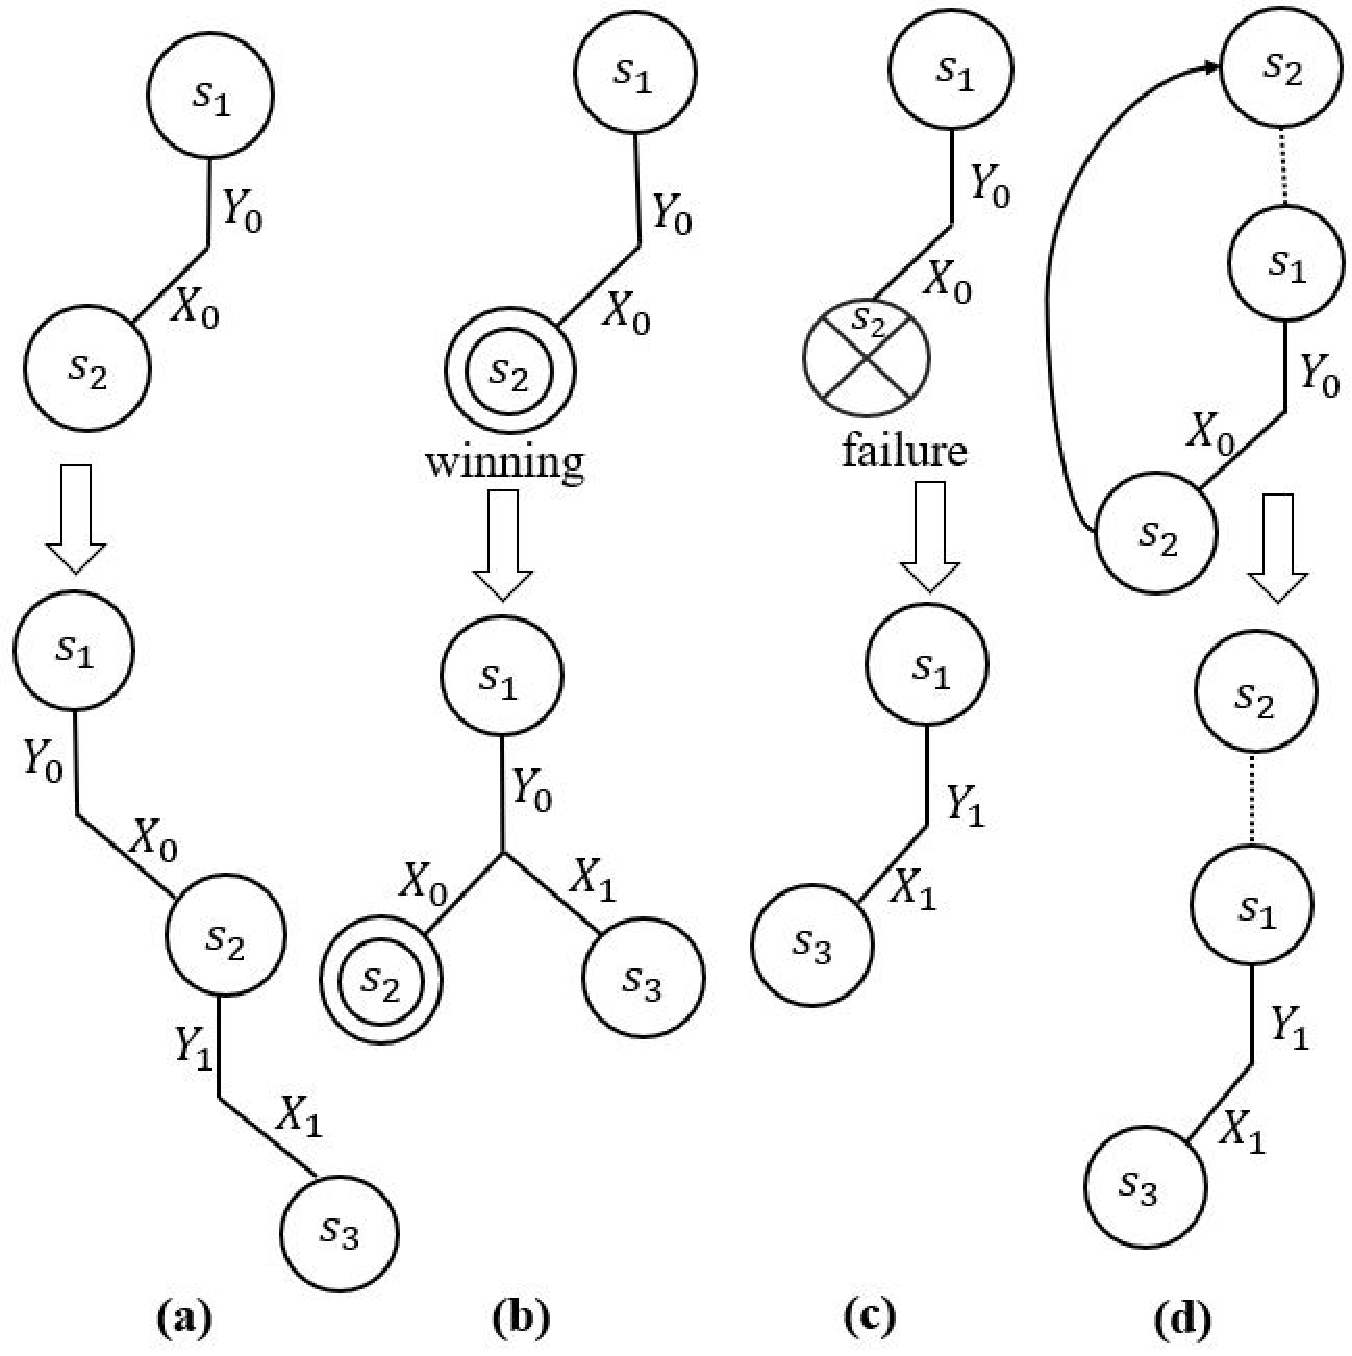
\includegraphics[scale=0.35]{demonstration.pdf}
    \caption{A demonstration of key operations for on-the-fly \ltlf synthesis.}
    \label{fig:demonstration}
\end{figure}




\section{Approach Overview}
This section presents the high-level ideas behind both the pre-processing and on-the-fly synthesis techniques. The pre-processing aims to determine the synthesis result directly based on the input formula and the input/output pair. First of all, it is trivial to know that the formula cannot (resp. can) be realizable if it is unsatisfiable (resp. valid). Therefore, one can run the satisfiability checkers, such as \aaltaf\citep{LRPZV19}, to check the satisfiability of the input formula before synthesis, ruling out the meaningless instances (Theorem \ref{thm:sat-syn}). Next, for an \ltlf formula with the atomic set $\mathcal{P} = \X\cup\Y$, if there is $Y\in 2^{\Y}$ such that $Y\models\phi$ is true ($Y$ being considered as a length-one finite trace), we can know that $\phi$ is realizable~(Theorem \ref{thm:winning-1}). Consider $\phi = \G (a\vee b)$ with $\X=\{a\}$ and $\Y=\{b\}$ as an example. Since $\{b\}\models\phi$ is true, $\phi$ is realizable. 
For an unrealizable formula $\phi$, we first define the \emph{projection} (Definition \ref{def:fp}), i.e., $\phi|_{\mathcal{P}_{\phi}}$, which is a Boolean formula including all first-position elements of traces accepted by $\phi$. Then, if there is no $Y\in 2^{\Y}$ such that $Y\models\phi|_{\mathcal{P}_{\phi}}$ is true, we can conclude that $\phi$ is unrealizable (Theorem \ref{thm:failure-1}). For instance, consider $\phi = \G (a\wedge b)$ with $\X=\{a\}$ and $\Y=\{b\}$. $\phi$ is determined as unrealizable even without constructing the corresponding \dfa. 
\iffalse
Finally, we introduce a stronger but easier-implementing version of Theorem \ref{thm:failure-1}, saying that if there exists $X\in 2^{\X}$ such that $X\models\phi|_{P_{\phi}}$ is not true, then $\phi$ is unrealizable (Theorem \ref{thm:failure-2}).  
\fi

We apply the \SAT-based technique presented in \cite{LRPZV19} that constructs automata (\NFA) states on the fly, to solve the synthesis problem. Given initial state $\phi$ (essentially a formula), the technique can generate a \emph{propositional assignment}, which includes one transition information starting from the state $\phi$. We adapt this technique accordingly such as to generate one transition for the transition-based \DFA~(\tdfa, a variant of \dfa that is better for on-the-fly construction). Then, the new methodology creates \tdfa states in four different ways as shown in Figure \ref{fig:demonstration}. From current state $s_1$, our approach creates state $s_2$ by fixing $Y_0\in 2^{\Y}$ and enumerating $X\in 2^{\X}$ (currently is $X_0$). After that,
\begin{itemize}
    \item[(a)]  if $s_2$ cannot be recognized as winning or failure, the DFS~(Depth-first Search) strategy is applied to create a new state $s_3$;
    \item[(b)] if $s_2$ is recognized as winning, another $X\in 2^{\X}$ (here is $X_1$) is selected by fixing $Y_0$, obtaining a new state $s_3$. If all successor states are winning, then $s_1$ is winning;
    \item[(c)] if $s_2$ is recognized as failure, another $Y\in 2^{\X}$ (here is $Y_1$) is selected and $Y_0$ is ruled out from the winning strategy in current search. If no more $Y$ can be selected, $s_1$ is a failure state;
    \item[(d)] if $s_2$ has been visited already, i.e., a loop is found during the state computation, we can prove that choosing $Y_0$ cannot belong to the winning strategy in current search, and another $Y\in 2^{\X}$ (here is $Y_1$) has to be selected. 
\end{itemize}

One can see that our on-the-fly approach is able to return either realizable or unrealizable result before the whole \dfa is constructed. 

\begin{figure}
    \centering
    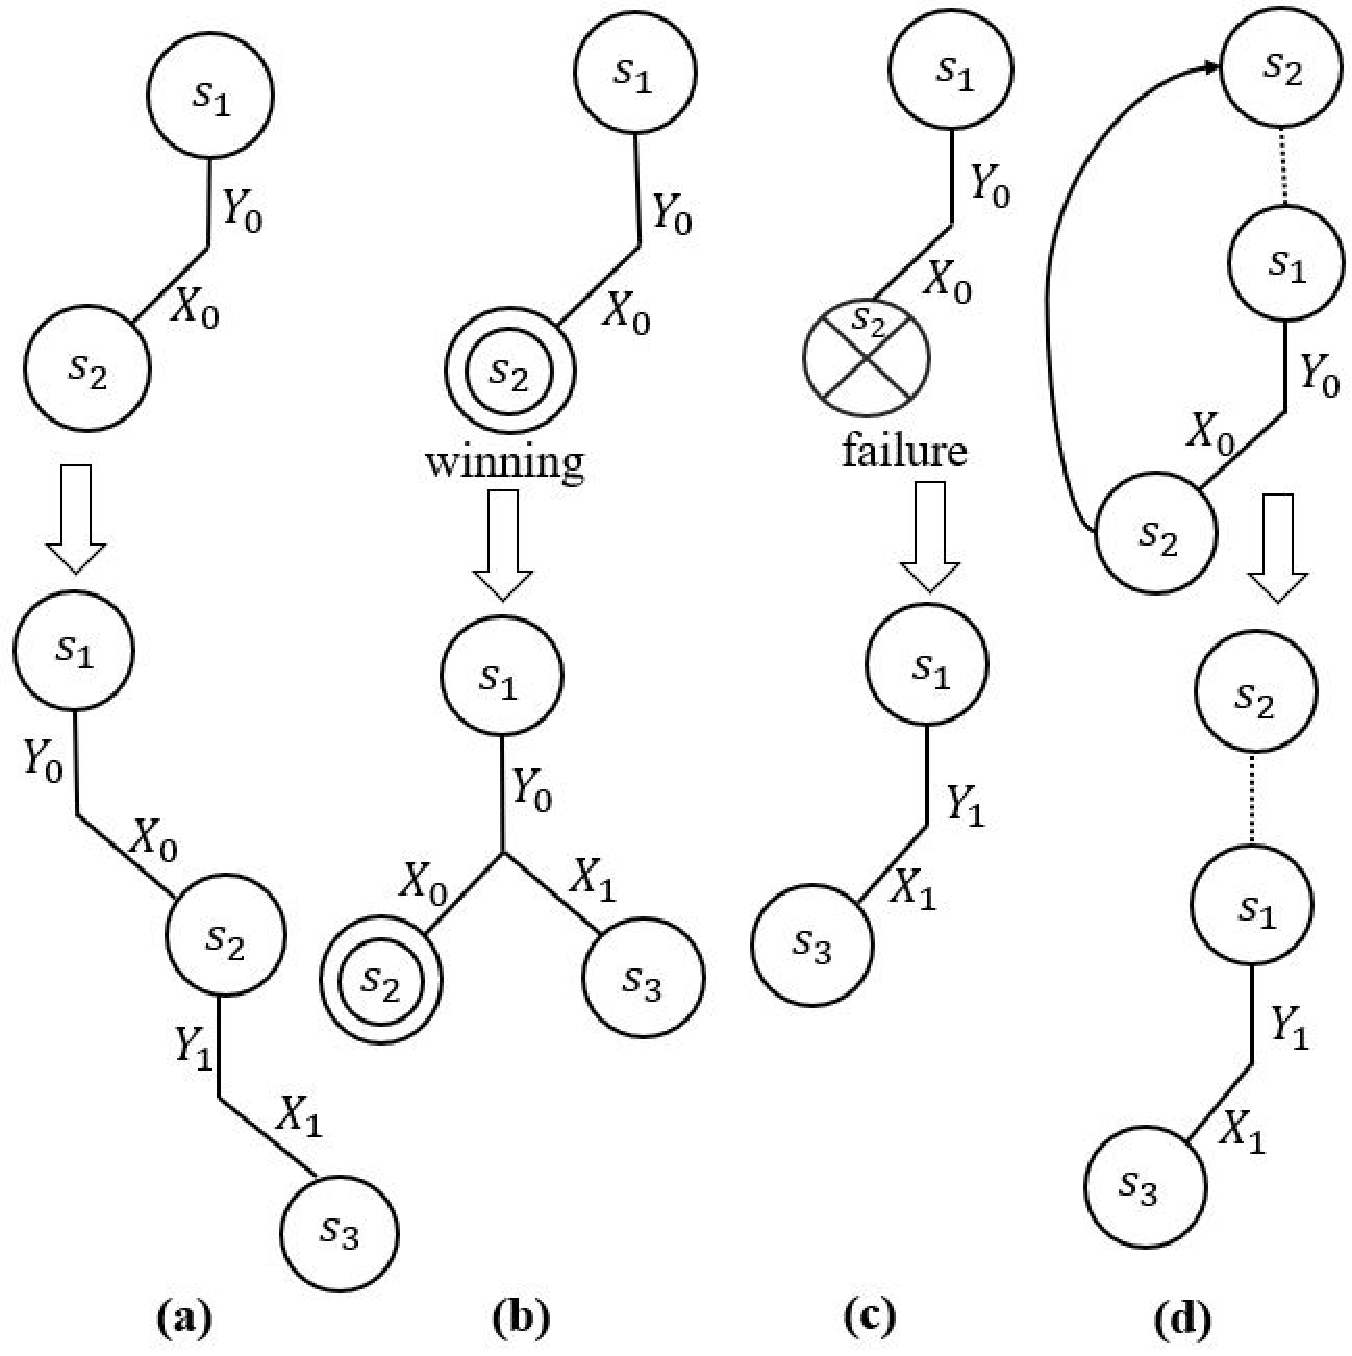
\includegraphics[scale=0.35]{demonstration.pdf}
    \caption{A demonstration of key operations for on-the-fly \ltlf synthesis.}
    \label{fig:demonstration}
\end{figure}




%\section{Pre-processing Techniques for \ltlf Synthesis}
In this section, we introduce three pre-processing techniques for \ltlf synthesis, which can be evaluated immediately on the given \ltlf formula w.r.t. the atomic set $\P=\X\cup\Y$. First, the following Lemma is straightforward according to the \ltlf semantics and Definition \ref{def:synthesis}.

\begin{theorem}\label{thm:sat-syn}
	If the \ltlf formula $\phi$ is unsatisfiable, then $\phi$ is unrealizable; If $\phi$ is valid, then $\phi$ is realizable.
\end{theorem}
Theorem~\ref{thm:sat-syn} suggests that an unsatisfiable/valid \ltlf formula is not quite useful as a synthesis specification in practice. 
To that end, an extant \ltlf-satisfiability solver, e.g., \aaltaf~\cite{LRPZV19}, can be used to check the satisfiability/validity of the formula before synthesis. We now define the $\satOnce$ predicate for further use. 

\begin{definition}\label{def:satOnce}
Given an \ltlf formula $\phi$ and $\omega \in 2^{\P}$, we define the predicate $\satOnce (\omega, \phi)$ is true iff 
\begin{itemize}
	\item $\phi$ is $\tt$; or
	\item $\phi$ is an atom and $\phi \in \omega$; or 
	\item $\phi = \neg\psi$ and $\neg \satOnce (\omega, \psi)$ is true; or
	\item $\phi = \phi_1\wedge\phi_2$ and $\satOnce (\omega, \phi_1)$ and $\satOnce (\omega, \phi_2)$ are true; or
	\item $\phi = \phi_1\vee\phi_2$ and $\satOnce (\omega, \phi_1)$ or $\satOnce (\omega, \phi_2)$ is true; or
	\item $\phi = \phi_1\U\phi_2$ or $\phi = \phi_1\R\phi_2$ and $\satOnce (\omega, \phi_2)$ is true.
\end{itemize} 
\end{definition}

Notably, $\satOnce (\omega, \ocircle\psi)$ can never be true, while $\satOnce (\omega, \N\psi)$ is always true. Based on Definition \ref{def:satOnce} and the semantics of \ltlf formulas, the lemma below is straightforward. 

\begin{lemma}\label{lem:satOnce}
Given an \ltlf formula $\phi$ and $\omega\in 2^{\P}$, $\satOnce (\omega, \phi)$ is true iff $\omega\models\phi$ holds.
\end{lemma}
In fact, Definition \ref{def:satOnce} can be considered as the simplified version of \ltlf semantics in which the length of the finite trace is restricted to be one. Definition \ref{def:satOnce} is provided as a better option for the implementation purpose. 

\begin{theorem}\label{thm:winning-1}
Given an \ltlf formula $\phi$ with alphabet $\X\cup \Y$, if there exists $Y\in 2^{\Y}$ such that $\satOnce (Y, \phi)$ is true, then $\phi$ is realizable. 
\end{theorem}
\begin{proof}
From Lemma \ref{lem:satOnce}, $\satOnce (Y, \phi)$ is true implies that $Y\models\phi$ is true. As a result, for every $X\in 2^{\X}$, $X\cup Y\models\phi$ is true, providing that $\X\cap \Y=\emptyset$. Therefore, there exists a strategy $g$ with $g(\epsilon) = Y$ such that for every $X\in 2^{\X}$ it holds that $X\cup g(\epsilon)\models\phi$. According to Definition \ref{def:synthesis}, $g$ is a winning strategy for the system and $\phi$ is realizable.
\end{proof}

Consider the formula $a\U b$ with $\X=\{a\}$ and $\Y=\{b\}$ as an example. Let $Y= \{b\}$ and since $\satOnce (Y, a\U b)$ is true, $\phi$ is realizable according to Theorem~\ref{thm:winning-1}. It is easy to induce that Theorem~\ref{thm:winning-1} can be extremely helpful for the synthesis instances like $\psi\U b$ with $\Y=\{b\}$, under which the realizable result can be achieved by Theorem~\ref{thm:winning-1} directly without further automata construction. This advantage may potentially lead to an exponential better performance, which will be discussed in the experimental section later. Next, we introduce the concept of \emph{formula projection} for the pre-processing of unrealizable formulas. 

\begin{definition}[Formula Projection]\label{def:fp}
Given an \ltlf formula $\phi$ in \NNF with the atomic set $\P$, we define its projection under $\P$, denoted as $\phi |_\P$, is a Boolean formula as follows:
\begin{itemize}
	\item $\phi|_\P = \phi$ if $\phi$ is $\tt$, $\ff$ or a literal;
	\item $\phi|_\P = \tt$ if $\phi = \ocircle\psi$ or $\phi = \N\psi$;
	\item $\phi|_\P = \phi_1|_\P \wedge \phi_2|_\P$ if $\phi = \phi_1\wedge\phi_2$;
	\item $\phi|_\P = \phi_1|_\P \vee \phi_2|_\P$ if $\phi = \phi_1\vee\phi_2$;
	\item $\phi|_\P = \phi_1|_\P \vee \phi_2|_\P$ if $\phi = \phi_1\U\phi_2$;
	\item $\phi|_\P = \phi_2|_\P$ if $\phi = \phi_1\R\phi_2$.
\end{itemize}
\end{definition}

\begin{lemma}\label{lem:fp}
Given an \ltlf formula $\phi$ and a finite trace $\eta$, $\eta\models\phi$ implies that $\eta[0]\models\phi|_\P$.
\end{lemma}
The proof can be done by induction over the structure of $\phi$, which is omitted here. Lemma \ref{lem:fp} indicates that $\phi|_\P$ is sufficient to capture all the first-position elements of $\phi$'s accepting traces. Inspired by that, we have the following theorem that can help with identifying a formula being unrealizable. 

\begin{theorem}\label{thm:failure-1}
Given an \ltlf formula $\phi$ with the atomic set $\X\cup \Y$, if there does not exists $Y\in 2^{\Y}$ such that $Y\models \phi|_{\X\cup\Y}$, then $\phi$ is unrealizable. 
\end{theorem}
\begin{proof}
Assume $\phi$ is realizable. According to Definition \ref{def:synthesis}, there exists a winning strategy $g$ such that for an arbitrary infinite sequence $X_0,X_1,\ldots\in (2^{\X})^{\omega}$, there exists $k\geq 0$ such that $\rho=(X_0\cup g(\epsilon)),(X_1\cup g(X_0)), \ldots, (X_k\cup g(X_{k-1}))$ satisfies $\phi$. Let $Y = g(\epsilon)$, and based on Lemma \ref{lem:fp}, we have that $Y\cup X_0\models \phi|_{\X\cup\Y}$ for every $X_0\in 2^{\X}$. As the consequence, it is required that $Y\models \phi|_{\X\cup\Y}$ is true. However, we already know that $Y\models \phi|_{\X\cup\Y}$ does not hold for any $Y\in 2^{\Y}$, which causes the contradiction. Therefore, we prove that $\phi$ is unrealizable.
\end{proof}

Consider formula $\phi= \G (a\wedge b)\wedge \G (c\wedge d)$ with $\X=\{a,c\}$ and $\Y=\{b,d\}$ as an example. From Definition~\ref{def:fp}, we have that $\phi|_\P=(a\wedge b\wedge c\wedge d)$. Obviously, $Y\models \phi|_\P$ does not hold for any $Y\in 2^{\Y}$. We can conclude that $\phi$ is unrealizable based on Theorem~\ref{thm:failure-1}. In general, the performance of the traditional synthesis approach for $\phi= \G (a\wedge b)\wedge \G (c\wedge d) \wedge\psi$ with $\X=\{a,c\}\cup \P_{\psi}$ and $\Y=\{b,d\}$ (assume $\P_{\psi}$ is the atomic set of $\psi$ and $\P_{\psi} \cap \{a,b,c,d\} = \emptyset$) can decrease exponentially w.r.t. the size of $\psi$, while that of the synthesis based on Theorem \ref{thm:failure-1} can escape from the drawback. 

\iffalse
\begin{theorem}\label{thm:failure-2}
	Given an \ltlf formula $\phi$ with the atomic set $\X\cup \Y$, if there exists $X\in 2^{\X}$ such that $X\models \phi|_{\X\cup\Y}$ does not hold, then $\phi$ is unrealizable. 
\end{theorem}
\begin{proof}
Assume $\phi$ is realizable. According to Definition \ref{def:synthesis}, there exists a winning strategy $g$ such that for an arbitrary infinite sequence $X_0,X_1,\ldots\in {2^{\X}}^{\omega}$, we can find $k\geq 0$ such that $\rho=(X_0\cup g(\epsilon)),(X_1\cup g(X_0)), \ldots, (X_k\cup g(X_{k-1}))$ satisfies $\phi$. Let $Y = g(\epsilon)$, and based on Lemma \ref{lem:fp}, we have that $Y\cup X_0\models \phi|_{\X\cup\Y}$ for every $X_0\in 2^{\X}$. However, we already have that there exists $X\in 2^{\X}$ (Let $X_0$ be such $X$) such that $X\not\models \phi|_{\X\cup\Y}$ holds, which implies that $X\cup Y\models \phi|_{\X\cup\Y}$ does not hold for any $Y\in 2^{\Y}$. This contradicts the assumption, leading to that $\phi$ is unrealizable.
\end{proof}

Theorem \ref{thm:failure-2} can be treated as a stronger version of Theorem \ref{thm:failure-1}, since it is not hard to see that Theorem \ref{thm:failure-2} is true implies Theorem \ref{thm:failure-1} is true. For the example above ($\phi= \G (a\wedge b)\wedge \G (c\wedge d)$ with $\X=\{a,c\}$ and $\Y=\{b,d\}$), the unrealizable result can also be deduced from Theorem \ref{thm:failure-2}. Nonetheless, Theorem \ref{thm:failure-2} is kept in our implementation as it can cost less than Theorem \ref{thm:failure-1} to determine the unrealizability, considering that every $Y\in 2^{\Y}$ has to be enumerated in Theorem \ref{thm:failure-1} while enumerating every $X\in 2^{\X}$ may not be necessary in Theorem \ref{thm:failure-2}.
\fi

\section{On-the-fly Synthesis via \tdfa Games}
In this section, we first introduce the theoretic foundation of the on-the-fly \ltlf synthesis approach, which is based on solving a \tdfa (Transition-based \dfa) game. We present an algorithm that is able to generate \tdfa on the fly to implement the synthesis. \tdfa is a variant of \dfa that is better for performing on-the-fly construction. The definition of \tdfa is shown below. 
 
\begin{definition}[Transition-based \dfa]\label{def:tdfa}
A transition-based \dfa (\tdfa) is a tuple $\A = (\Sigma,S,s_0,\delta,T)$, where 
\begin{itemize}
    \item $\Sigma$ is a set of alphabet;
    \item $S$ is a set of states;
    \item $s_0\in S$ is the initial state;
    \item $\delta:S\times\Sigma\hookrightarrow S$ is the transition function, which is a partial function, i.e. $\delta (s, \omega)\in S$ or $\delta (s, \omega)$ is undefined for $s\in S$ and $\omega\in {\Sigma}$;
    \item $T \subseteq \delta$ is the set of accepting transitions.
\end{itemize}
\end{definition}

The run $r$ of $\A$ on a finite trace $\eta=\omega_0, \omega_1,\cdots, \omega_n \in \Sigma^+$ is a finite state sequence $r = s_0,s_1,\ldots,s_{n+1}$ such that $s_0$ is the initial state and $\delta (s_i, \omega_i) = s_{i+1}$ is true for $0\leq i \leq n$.
The trace $\eta$ is accepted by $\A$ iff the corresponding run $r$ ends with an accepting transition, i.e., $\delta (s_n, \omega_n) = s_{n+1}$ is in $T$. For the sake of simplicity, we denote transition $\delta (s_1, \omega) = s_2$ as $s_1\tran{\omega}s_2$.

\begin{lemma}\label{lem:tdfa}
The \tdfa is as expressive as the \dfa.
\end{lemma}
\begin{proof}
	($\Leftarrow$:) A \dfa can be trivially converted to its equivalent \tdfa by marking all transitions leading to accepting states as accepting transitions. Therefore, every trace that is accepted by the \dfa is also accepted by this \tdfa.
	
	($\Rightarrow$:) We first convert a \tdfa to an \nfa by adding a new state $ns$, which is marked as the unique accepting state of this \nfa. Later, we create a transition $s\tran{\omega}ns$ if transition $s\tran{\omega}s'$ is an accepting transition of the \tdfa. Therefore, every trace that is accepted by the \tdfa is also accepted by this \nfa. From the constructed \nfa, one can trivially generate the equivalent \dfa by the subset construction. 
\end{proof}


According to \cite{GV13}, every \ltlf formula can be converted to a \dfa that accepts exactly the same language as the \ltlf formula. Therefore, it is straightforward that there is also a \tdfa for every \ltlf formula such that they accept the same language. 

In this paper, we present a dedicated \SAT-based \ltlf-to-\tdfa construction technique for on-the-fly synthesis. The \SAT-based \ltlf-to-automata construction technique was first introduced in \cite{LRPZV19}, and we follow the methodology presented in the literature. Given an \ltlf formula $\phi$, this technique is able to generate a \emph{propositional assignment} $A$ of $\phi$ such that $A$ includes the information of a transition in the corresponding \NFA. For more details,
%\cite{LRPZV19} provides a way to generate a \emph{propositional assignment} $A$ of $\phi$ such that $A$ includes the information of one transition for the \NFA generation. 
we refer to the literatrue \cite{LRPZV19} and here we just use $\SAT(\phi)$ to denote such process. Assume $A = \SAT(\phi)$ is a \emph{propositional assignment} returned by the \SAT-based technique, we use $L(A)$ to denote the transition label, which is represented as a Boolean formula, and $\mathbf{next}(A)$ to denote the successor state of $\phi$. $\phi$ represents the current state.
The \tdfa construction can be achieved as follows.  

\begin{definition}[\ltlf-to-\tdfa]\label{def:ltlf2dfa}
Given an \ltlf formula $\phi$, the corresponding \TDFA ${\A_{\phi}}$ is a tuple $(\Sigma, S, \delta, s_0, T)$ s.t.
\begin{itemize}
	\item $\Sigma = 2^{\L}$ is the set of alphabet and $\L$ is the literal set of $\phi$;
	\item $S\subseteq 2^{2^{\cl(\phi)}}$ is the set of states;
	\item $\delta:  S \times \Sigma \hookrightarrow S$ is the partial transition function, where $s_2 = \delta(s_1, \omega) \mbox{ holds}$ iff $s_2=\{\mathbf{next}(A) | A\in\{\SAT(s_1)\}\textit{ and }\omega \models L(A)\}$ for $\omega \in \Sigma$;
	\item $s_0 = \{\{\phi \}\}$ is the initial state;
	\item $T\subseteq \delta$ is the set of accepting transitions. A transition $s_1\tran{\omega}s_2$ is in $T$ iff $\omega\models s_1$ holds. 
\end{itemize}

\end{definition}

From Definition \ref{def:ltlf2dfa}, a \tdfa state $s$ is a set of set of subformulas of the input formula $\phi$. \textbf{For the description convenience, we mix the usage of the state and the formula in the following.} That is to say, $s$ represents the formula $\bigvee_{q\in s}\bigwedge_{\psi\in q} \psi$, and vice versa. The following theorem guarantees the correctness of the \tdfa construction shown in Definition \ref{def:ltlf2dfa}. 

\begin{theorem}\label{thm:ltlf2tdfa}
Given an \ltlf formula $\phi$ and the \tdfa ${\A_{\phi}}$ constructed by Definition \ref{def:ltlf2dfa}, a finite trace $\eta\models\phi$ holds iff $\eta$ is accepted by ${\A_{\phi}}$. 
\end{theorem}
The proof of this theorem requires more details from \cite{LRPZV19}, which are referred to the literature. %are shown in Appendix. 
As long as we obtain the \tdfa of the given \ltlf formula, the synthesis problem can be reduced to a \tdfa game.

\begin{definition}[\tdfa Game]\label{def:tdfa-game}
	A \tdfa game is a two-player game over a \tdfa $\A = (2^{\X \times \Y}, S, s_0, \delta, T)$ such that 
	\begin{itemize}
		\item $2^{\X \times \Y}$ is the alphabet of the game, where $\X$ and $\Y$ are two disjoint sets of variables that are controlled by the environment and system respectively;
		\item $S$ is the set of states;
		\item $s_0$ is the initial state;
		\item $\delta:S\times 2^{\X \times \Y}\hookrightarrow S$ is the partial transition function, i.e. $\delta (s, X\cup Y)$ is in $S$ or undefined for $s\in S$, $X\in 2^{\X}$ and $Y\in 2^{\Y}$;
    \item $T \subseteq \delta$ is the set of accepting transitions of the game, visiting which the system can terminate the game and declare as winning.
	\end{itemize}
\end{definition}
To coordinate with \ltlf synthesis, we focus on the \textbf{System-first} \tdfa game as well. We say a \tdfa game is \emph{winning} for the system iff there is a system winning strategy $g: (2^{\X})^*\rightarrow 2^{\Y}$ such that for an arbitrary infinite environment sequence $X_0,X_1,\ldots\in (2^{\X})^{\omega}$, there is $k > 0$, such that the corresponding run $r $ on the finite trace $ (X_0\cup g(\epsilon)), (X_1\cup g(X_0)),\ldots, (X_k\cup g(X_{k-1}))$ is accepted by $\A$.
In the following, we define system \emph{winning} and \emph{failure} states of a \tdfa game.

\begin{definition}[System Winning/Failure State]\label{def:winning_failure_state}
\label{def:win_st}
For a \tdfa game over $\A =(2^{\X \times \Y},S,s_0,\delta,T)$, $s\in S$ is a system winning state iff there is $Y \in 2^\Y$ such that for every $X \in 2^\X$, either $\delta(s,X\cup Y)=s'$ is an accepting transition or $s'$ is a winning state. Moreover, we say $s$ is a system failure state iff it is not a system winning state.
\end{definition}

The following lemma is deducible from Definition \ref{def:winning_failure_state} instantly and can be used as an easy check in the algorithm. 

\begin{lemma}
For a \tdfa game $\A =(2^{\X \times \Y},S,s_0,\delta,T)$ and state $s\in S$, 
\begin{enumerate}
	\item $s$ is a system winning state if there is $Y \in 2^\Y$ such that for every $X \in 2^\X$, $\delta(s,X\cup Y)=s'$ is an accepting transition;
	\item $s$ is a failure state if for every $Y \in 2^\Y$, there is $X \in 2^\X$ such that $\delta(s,X \cup Y)$ is undefined.
\end{enumerate} 
\end{lemma}

Informally speaking, a system winning state is a state if all of its out-going transitions are defined, and are either accepting or leading to some winning state. To the opposite, a system failure state is a state which has some out-going transitions undefined, or has a part of the transitions leading to the failure states. The next theorem shows how to use the winning/failure state to determine the \tdfa game.
 

\begin{theorem}\label{thm:winning-and-failure}
Given a \tdfa game $\A =(2^{\X \times \Y},S,s_0,\delta,T)$, $s_0$ is a system winning state iff the system wins the game.
\end{theorem}
The theorem can be proved by induction over the states of \tdfa based on Definition \ref{def:tdfa-game} and \ref{def:winning_failure_state}. Now, we present the main theorem for our synthesis approach. 
%Based on Definitions \ref{def:winning_failure_state}, the follow theorem is also straightforward.

\begin{theorem}\label{thm:system-and-game}
For an \ltlf formula $\phi$ with $\X$ and $\Y$, let $\A =(2^{\X \times \Y},S,s_0,\delta,T)$ be the corresponding \tdfa game description. $s_0$ is a system winning state iff $\phi$ is realizable.
\end{theorem}
\begin{proof}
$(\Rightarrow)$ Since $s_0$ is a system winning state, there is a system winning strategy $g: (2^\X)^* \rightarrow 2^\Y$ such that for an arbitrary infinite sequence $X_0,X_1,\ldots\in (2^{\X})^{\omega}$, there exists $k > 0$ such that the run of $\A$ on the finite trace $\rho=(X_0\cup g(\epsilon)),(X_1\cup g(X_0)), \ldots, (X_k\cup g(X_{k-1}))$  is an accepting run. Therefore, $\rho \models \phi$ holds and $g$ is the system winning strategy.

$(\Leftarrow)$ If $\phi$ is realizable, then there is a system winning strategy $g: (2^\X)^* \rightarrow 2^\Y$ such that for an arbitrary infinite sequence $X_0,X_1,\ldots\in (2^{\X})^{\omega}$, there exists $k > 0$ such that the finite trace $\rho=(X_0\cup g(\epsilon)),(X_1\cup g(X_0)), \ldots, (X_k\cup g(X_{k-1}))$ satisfies $\phi$. The run of $\A$ on $\rho$ is thus an accepting run. Therefore, $s_0$ is a system winning state with winning strategy $g$.
\end{proof}

An important question is raised, which is how to determine whether the initial state is a \emph{winning/failure state}? The classical synthesis approach \cite{GV15} first constructs the whole \dfa w.r.t. the input \ltlf formula, and then performs a backward fixpoint computation. The fixpoint is initialized as the set of accepting states, visiting which the system obviously wins the game. The fixpoint computation then iteratively collects new states from which the system is able to reach an already-defined winning state, no matter how the environment behaves. The computation terminates as soon as we reach the fixpoint, i.e., no more winning states can be collected. The system wins the game if the initial state $s_0$ is in the winning set. The main drawback of this approach is that the winning states can only be collected after the full \dfa is obtained.  

We present in this paper a new technique that is able to collect the set of system winning states and synthesize the system winning strategy on the fly. The algorithm \tool, which is shown in Algorithm \ref{alg:win}, describes the main procedure of this technique. Comments are blue-colored for better understanding. We summarize the crucial parts of the technique as follows.


\begin{algorithm}[h]
\caption{\tool: Compute the winning strategy on the fly}
\label{alg:win}
	\begin{algorithmic}[1]
		\REQUIRE{\ltlf formula $\phi$ with $\X$ and $\Y$;}
		\ENSURE{$\Omega=\{\langle s, Y, \{\langle X, s'\rangle\}\rangle\}$ if $\phi$ is realizable, otherwise return $\emptyset$;\COMMENT{\textcolor{blue}{$s,s'\in S$, $X\in 2^{\X}$ and $Y\in 2^{\Y}$}}}
		
		\STATE Let $\langle ret, \Omega\rangle\coloneqq preprocess(\phi, \X, \Y)$;\COMMENT{\textcolor{blue}{Check by the pre-processing techniques at first}}\label{alg:win:preprocess-start}
		\IF{$ret\neq unknown$}
    		\RETURN $\Omega$;
    	\ENDIF\label{alg:win:preprocess-end}
    	\WHILE{true\COMMENT{\textcolor{blue}{Enumerate $Y$ inside}}}\label{alg:win:Yloop-start}
    		\STATE $\langle \omega,s\rangle\coloneqq getTransition(\phi,\emptyset)$;\COMMENT{\textcolor{blue}{Get  $\phi\tran{\omega}s$}}
    		\IF{$\langle \omega,s\rangle =\emptyset$}
        		\RETURN $\emptyset$;
    		\ENDIF
    	\STATE Let $\phi'\coloneqq \phi$ and $r \coloneqq \langle \phi, Y=\omega|_{\Y}, Q=\{\langle \omega|_{\X}, s\rangle\}\rangle$;
    	\STATE Push $r$ into $\Omega$;
    	\WHILE{true\COMMENT{\textcolor{blue}{Fix $Y=\omega|_{\Y}$, enumerate $X$ inside}}}\label{alg:win:Xloop-start}
        	\IF{$s$ has been generated\COMMENT{\textcolor{blue}{A loop is detected}}}\label{alg:win:loop-detect}
            	\BREAK;\COMMENT{\textcolor{blue}{This $Y$ cannot be a move in a winning strategy}}
            \ENDIF
        	\IF{$\omega\models \phi'$\COMMENT{\textcolor{blue}{An accepting transition is detected}}}
            	\STATE $\phi'\coloneqq \phi'\wedge(\neg(\omega|_{\X}))$;\COMMENT{\textcolor{blue}{Enumerate $X$}}
        	\ELSE
            	\STATE Let $\Omega'\coloneqq \tool(s, \X, \Y)$;\label{alg:win:recursive}
            	\IF{$\Omega'\not = \emptyset$\COMMENT{\textcolor{blue}{$s$ is a winning state}}}	
                	\STATE $\phi'\coloneqq \phi'\wedge(\neg(\omega|_{\X}))$;\COMMENT{\textcolor{blue}{Enumerate $X$}}
            	\ELSE
                	\BREAK;\COMMENT{\textcolor{blue}{The chosen $Y$ is not a move of a winning strategy}}
            	\ENDIF
        
        	\ENDIF
        	\STATE $\langle\omega',s'\rangle\coloneqq getTransition(\phi',\omega|_\Y)$;\COMMENT{\textcolor{blue}{Get the transition $\phi\tran{\omega'}s'$ such that $\omega|_{\Y}\subseteq \omega'$}}
        	\IF{$\langle\omega',s'\rangle=\emptyset$\COMMENT{\textcolor{blue}{Enumerating $X$ is finished}}}
            	\RETURN $\Omega$;\label{alg:win:loop-stop}
            \ELSE
            	\STATE Update $r=\langle \phi, Y, Q\rangle$ by pushing $\langle \omega'|_{\X}, s'\rangle$ into $Q$;
        	\ENDIF
    	\ENDWHILE\label{alg:win:Xloop-end}
    	\STATE Remove $r$ from $\Omega$;
    	\STATE $\phi\coloneqq \phi\wedge(\neg(\omega|_{\Y}))$;\COMMENT{\textcolor{blue}{Enumerate $Y$}}\label{alg:win:chooseY}
	\ENDWHILE\label{alg:win:Yloop-end}
	\end{algorithmic}
\end{algorithm}



The algorithm $\tool$ takes a tuple $(\phi, \X, \Y)$ as the input and returns a set $\Omega$ which represents the winning strategy  if $(\phi, \X, \Y)$ is realizable, or an empty set if unrealizable. Each element of $\Omega$ is in the form of $\langle s, Y, \{\langle X, s'\rangle\}\rangle$, where $s,s'\in S$, $X\in 2^{\X}$ and $Y\in 2^{\Y}$. Each element indicates that from state $s$, the system can take $Y$ as a move, such that no matter how the environment chooses $X \in 2^\X$, the next state $s'$ is also a system winning state, i.e., $s\tran{X\cup Y}s'$ is a transition of the \tdfa and $s'$ is a winning state as well.

\begin{algorithm}
\caption{Implementation of function \emph{getTransition}}\label{alg:getTransition}
	\begin{algorithmic}[1]
	\REQUIRE{\ltlf formula $\phi$, and a set of literals $assumption$;}
	\ENSURE{$\langle label,next\rangle$ such that $\phi\tran{label}next$ is a transition of the \tdfa, otherwise return $\emptyset$;}
	
	\STATE Let $label\coloneqq null$, $next \coloneqq null$;
	\STATE Let $\phi\coloneqq \phi\wedge\left(\bigwedge assumption\right)$;
	 \WHILE{true\COMMENT{\textcolor{blue}{Find $label$ such that $Y=label|_{\Y}$ satisfies $Y\models\phi|_{\X\cup\Y}$}}}\label{alg:getTransition:first-loop-start}
    	\STATE Let $A = \SAT (\phi)$;
    	\IF{$A=\emptyset$}
    		\BREAK;
    	\ENDIF
    	\IF{$A|_\Y\models \phi|_{\X\cup\Y}$}\label{alg:getTransition:feasible-check}
        	\STATE $label\coloneqq L(A)$;
        	\STATE $next\coloneqq \mathbf{next}(A)$;
        	\BREAK;\COMMENT{\textcolor{blue}{$Y=A|_{\Y}$ is found}}
    	\ENDIF
    	\STATE $\phi\coloneqq \phi\wedge\left(\neg\bigwedge A|_\Y\right)$;
	\ENDWHILE\label{alg:getTransition:first-loop-end}
	\STATE $\phi\coloneqq \phi\wedge label\wedge(\neg next)$;
	\WHILE{true\COMMENT{\textcolor{blue}{Fix $label$ and generate the successor state of $\phi$ in the \tdfa}}}\label{alg:getTransition:second-loop-start}
    	\STATE Let $A = \SAT(\phi)$;
    	\IF{$A=\emptyset$}
    		\BREAK;
    	\ENDIF
    	\STATE $next\coloneqq next\vee \mathbf{next}(A)$;
    	\STATE $\phi\coloneqq \phi\wedge(\neg (\mathbf{next}(A)))$;
	\ENDWHILE\label{alg:getTransition:second-loop-end}
	\IF{$label=null$ or $next=null$}
		\RETURN $\emptyset$;
	\ENDIF
	\RETURN $\langle label,next\rangle$;
	\end{algorithmic}
\end{algorithm}

\tool starts with the preprocessing techniques from Line \ref{alg:win:preprocess-start} to \ref{alg:win:preprocess-end}. The \emph{preprocess} function implements Theorem \ref{thm:sat-syn}-\ref{thm:failure-1}, and $\tool$ returns immediately if the function succeeds to determine $\phi$ is a winning or failure state. The loop from Line \ref{alg:win:Yloop-start} to \ref{alg:win:Yloop-end} aims to enumerate $Y\in 2^{\Y}$ inside, and it can terminate as long as a winning move $Y$ for the system is found (at Line \ref{alg:win:loop-stop}). Meanwhile, the loop from Line \ref{alg:win:Xloop-start} to \ref{alg:win:Xloop-end} has to enumerate every $X\in 2^{\X}$ before it can conclude the fixed $Y$ is indeed a winning move for the system. If the enumeration on $X$ is not successful, another $Y$ has to be chosen (at Line \ref{alg:win:chooseY}) and the above process repeats.

There are two points that need to be addressed clearly in the algorithm. Firstly, if the new transition $\phi\tran{\omega}s$ is not an accepting transition, $\tool$ will be invoked on $s$ recursively to determine whether $s$ is a winning state (at Line \ref{alg:win:recursive}). Secondly, if a loop is detected before $s$ can be determined as the winning state for the system (at Line \ref{alg:win:loop-detect}), the current chosen $Y$ cannot be a move in a winning strategy.  Assume the run of the \tdfa is $r=s,s_1,\ldots, s$. Starting from $s$, the environment can have the option to induce the same run as $r$, in which case the system can never win.  



The Algorithm \ref{alg:getTransition} is used to calculate a feasible transition in \tdfa. To enumerate $X$, we set the parameter \emph{assumption} that represents the current fixed $Y$. The first while loop (from Line \ref{alg:getTransition:first-loop-start} to Line \ref{alg:getTransition:first-loop-end}) aims to obtain a feasible label of a \tdfa transition. According to Theorem \ref{thm:failure-1}, when we get an assignment $A$ from the \SAT solver, we check whether $A|_\Y\models \phi|_{\X\cup\Y}$ holds~(Line \ref{alg:getTransition:feasible-check}) to determine whether this transition is feasible. The second while loop (from Line \ref{alg:getTransition:second-loop-start} to Line \ref{alg:getTransition:second-loop-end}) is to calculate all possible \NFA successors when fixing the labels of the transition so as to generate the \tdfa successor. In this loop, we fix the \emph{labels} each time and enumerate the \emph{next} part of the \NFA transition. If the first loop cannot find a feasible \tdfa transition, the $getTransition$ function returns $\emptyset$. 


\begin{figure*}[ht!]
% \subfigure{
\begin{minipage}{0.33\linewidth}
\centering
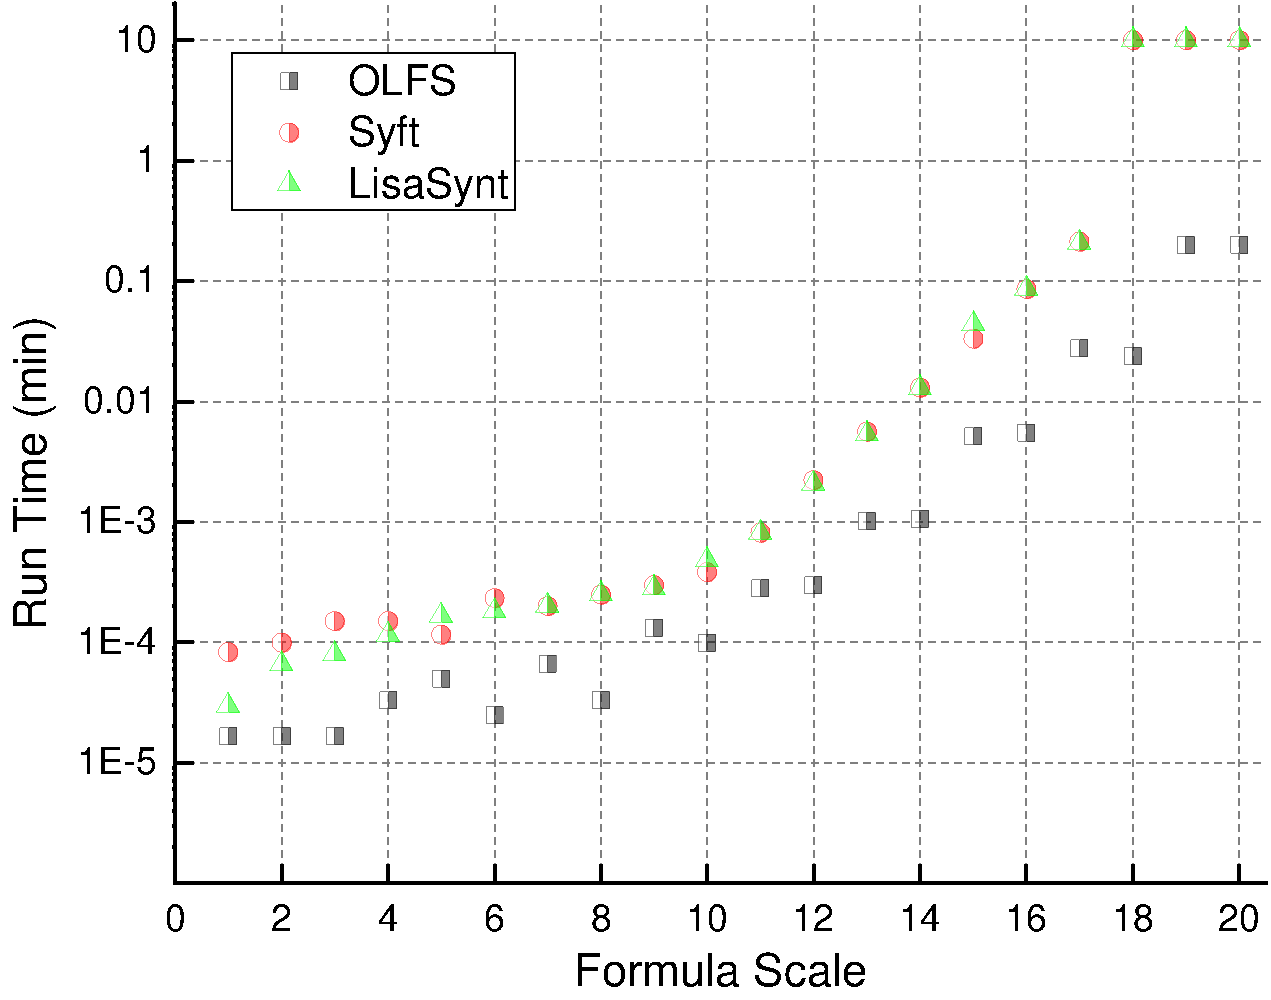
\includegraphics[width=5.5cm]{pic1_1.pdf}
    \caption{Results on the pattern formula $U (n) = p_1\U(p_2\U(...\U p_n))$.}
    \label{fig:preprocess-1}
\end{minipage}%
% }%
% \subfigure{
\begin{minipage}{0.33\linewidth}
\centering
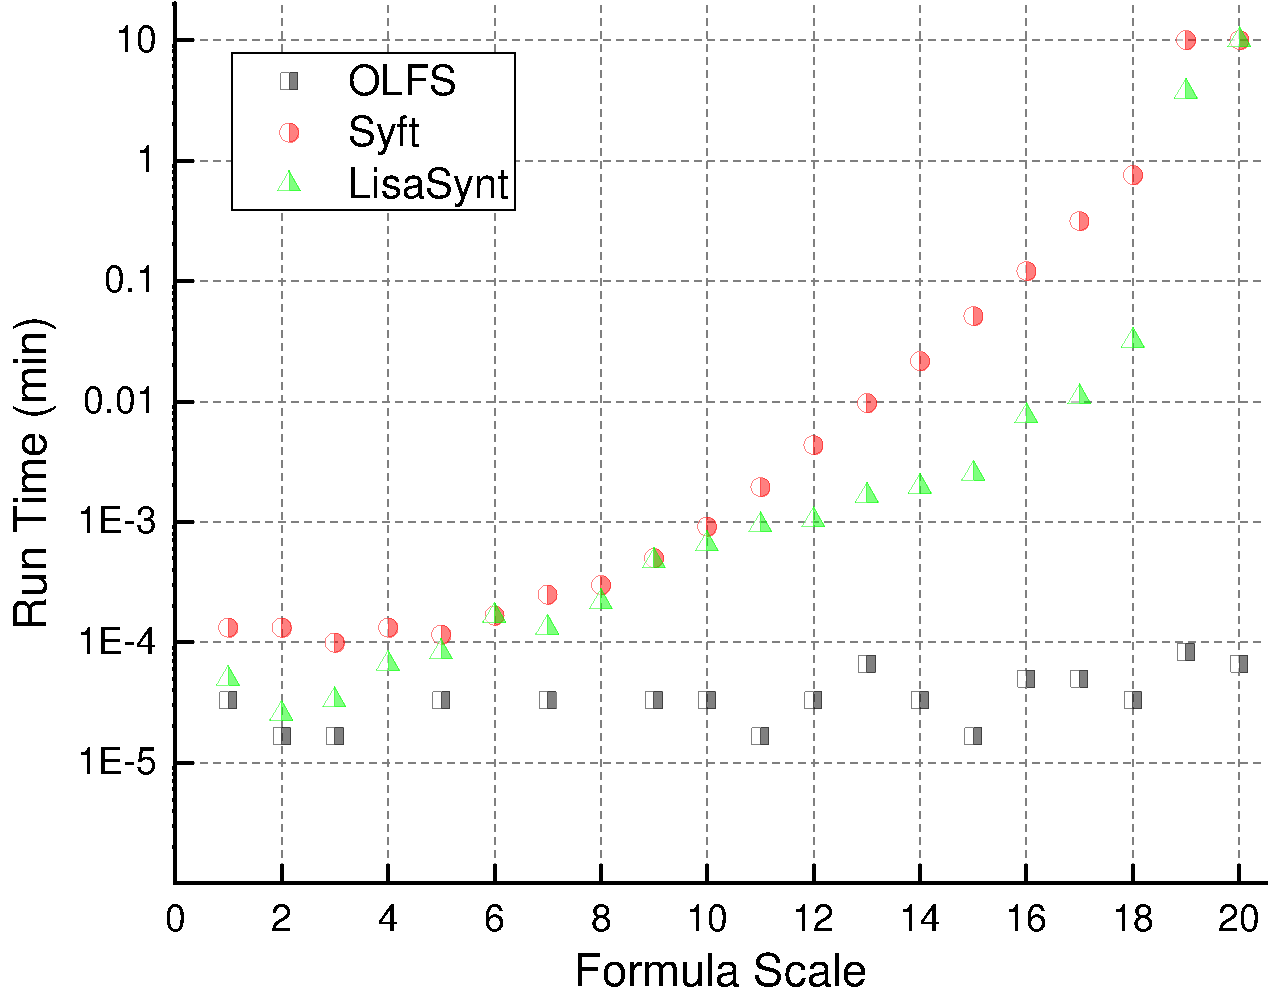
\includegraphics[width=5.5cm]{pic1_2.pdf}
    \caption{Results on the pattern formula $GF (n) = \G p_1\wedge(\bigwedge_{i=2\cdots n}\F p_i)$.}
    \label{fig:preprocess-2}
\end{minipage}%
% }%
% \subfigure{
\begin{minipage}{0.33\linewidth}
\centering
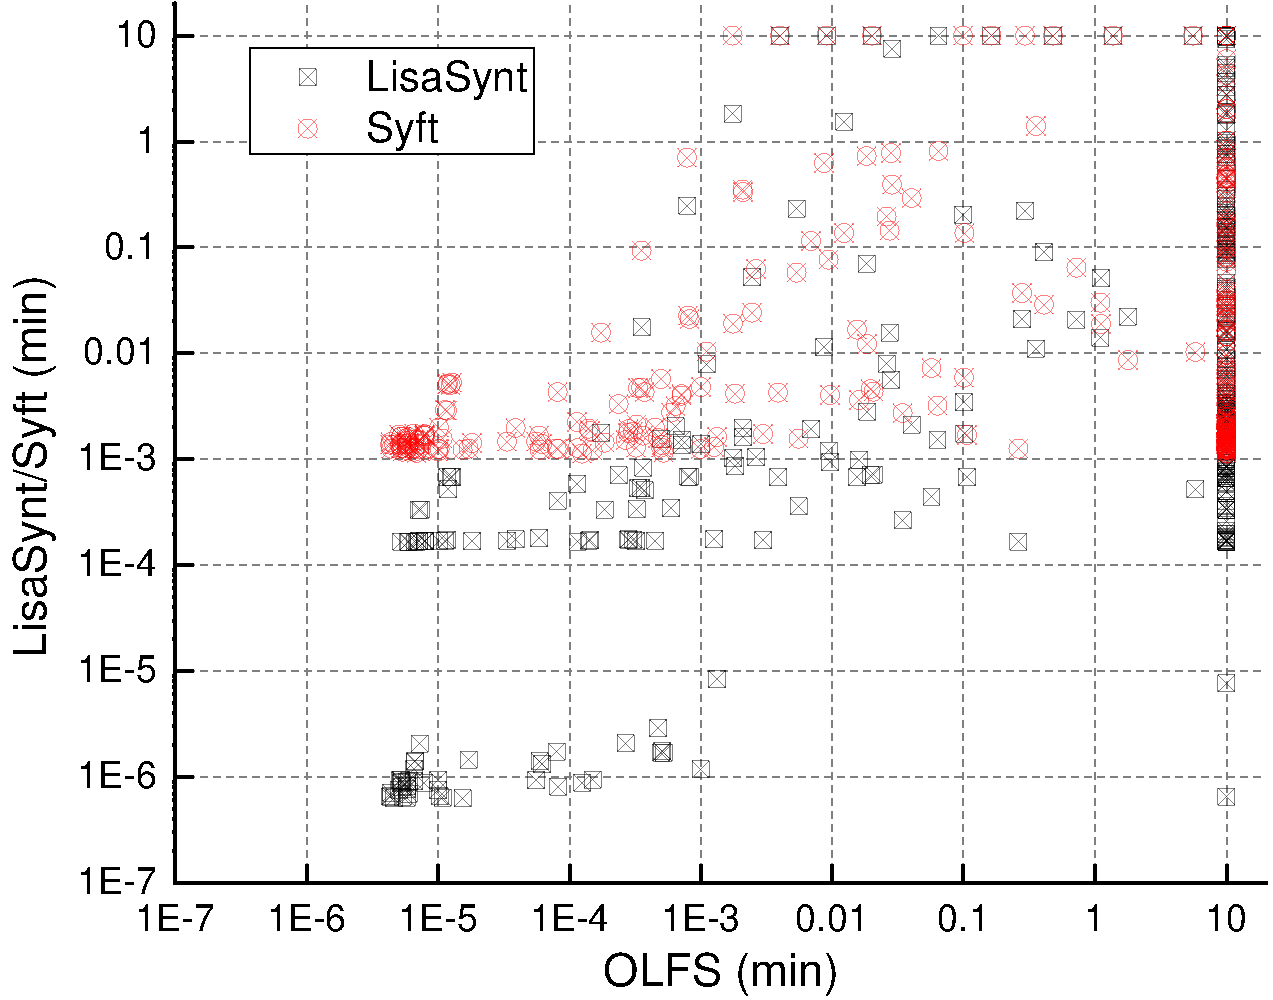
\includegraphics[width=5.5cm]{pic2.pdf}
    \caption{Results on the benchmarks from~\cite{BLTV20}.}
        \label{fig:otf}
\end{minipage}
% }%
\end{figure*}

Let $\Omega = \tool (\phi, \X, \Y)$ and we now define the strategy generator based on $\Omega$. Notably, our strategy generator only returns one winning strategy due to the on-the-fly construction, while the approach in \cite{GV15} is able to return all possible winning strategies. 

\begin{definition}[Strategy Generator]\label{def:transducer}
	The strategy generator for the \ltlf synthesis problem $(\phi, \X, \Y)$ is a transducer $\mathcal{T}_{\A}=(2^{\X\times\Y}, S, s_0, \xi, \sigma)$ such that
	\begin{itemize}
		\item $2^{\X\times\Y}$ is the alphabet of the transducer;
		\item $S = \{s| \langle s, Y, \{\langle X, s'\rangle\}\rangle \in\Omega\}\subseteq 2^{2^{\cl(\phi)}}$ is the set of states;
		\item $s_0 = \{\{\phi\}\}$ is the initial state;
		\item $\xi: S\times 2^{\X}\rightarrow 2^S$ is the transition function such that $\xi (s, X) = \{s' | \langle s, Y, \{\langle X, s'\rangle\}\rangle\in \Omega\}$;
		\item $\sigma: S\rightarrow 2^{\Y}$ is the output function such that $\sigma(s)=\{Y | \langle s, Y, \{\langle X, s'\rangle\}\rangle \in \Omega\}$.
	\end{itemize}
\end{definition}







\section{Pre-processing Techniques for \ltlf Synthesis}
In this section, we introduce three pre-processing techniques for \ltlf synthesis, which can be evaluated immediately on the given \ltlf formula w.r.t. the atomic set $\mathcal{P}=\X\cup\Y$. First, the following Lemma is straightforward according to the \ltlf semantics and Definition \ref{def:synthesis}.

\begin{theorem}\label{thm:sat-syn}
	If the \ltlf formula $\phi$ is unsatisfiable, then $\phi$ is unrealizable; If $\phi$ is valid, then $\phi$ is realizable.
\end{theorem}
Theorem~\ref{thm:sat-syn} suggests that an unsatisfiable/valid \ltlf formula is not quite useful as a synthesis specification in practice. 
To that end, an extant \ltlf-satisfiability solver, e.g., \aaltaf~\cite{LRPZV19}, can be used to check the satisfiability/validity of the formula before synthesis. We now define the $\satOnce$ predicate for further use. 

\begin{definition}\label{def:satOnce}
Given an \ltlf formula $\phi$ and $\omega \in 2^{\mathcal{P}}$, we define the predicate $\satOnce (\omega, \phi)$ is true iff 
\begin{itemize}
	\item $\phi$ is $\true$; or
	\item $\phi$ is an atom and $\phi \in \omega$; or 
	\item $\phi = \neg\psi$ and $\neg \satOnce (\omega, \psi)$ is true; or
	\item $\phi = \phi_1\wedge\phi_2$ and $\satOnce (\omega, \phi_1)$ and $\satOnce (\omega, \phi_2)$ are true; or
	\item $\phi = \phi_1\vee\phi_2$ and $\satOnce (\omega, \phi_1)$ or $\satOnce (\omega, \phi_2)$ is true; or
	\item $\phi = \phi_1\U\phi_2$ or $\phi = \phi_1\R\phi_2$ and $\satOnce (\omega, \phi_2)$ is true.
\end{itemize} 
\end{definition}

Notably, $\satOnce (\omega, \ocircle\psi)$ can never be true, while $\satOnce (\omega, \N\psi)$ is always true. Based on Definition \ref{def:satOnce} and the semantics of \ltlf formulas, the lemma below is straightforward. 

\begin{lemma}\label{lem:satOnce}
Given an \ltlf formula $\phi$ and $\omega\in 2^{\mathcal{P}}$, $\satOnce (\omega, \phi)$ is true iff $\omega\models\phi$ holds.
\end{lemma}
In fact, Definition \ref{def:satOnce} can be considered as the simplified version of \ltlf semantics in which the length of the finite trace is restricted to be one. Definition \ref{def:satOnce} is provided as a better option for the implementation purpose. 

\begin{theorem}\label{thm:winning-1}
Given an \ltlf formula $\phi$ with alphabet $\X\cup \Y$, if there exists $Y\in 2^{\Y}$ such that $\satOnce (Y, \phi)$ is true, then $\phi$ is realizable. 
\end{theorem}
\begin{proof}
From Lemma \ref{lem:satOnce}, $\satOnce (Y, \phi)$ is true implies that $Y\models\phi$ is true. As a result, for every $X\in 2^{\X}$, $X\cup Y\models\phi$ is true, providing that $\X\cap \Y=\emptyset$. Therefore, there exists a strategy $g$ with $g(\epsilon) = Y$ such that for every $X\in 2^{\X}$ it holds that $X\cup g(\epsilon)\models\phi$. According to Definition \ref{def:synthesis}, $g$ is a winning strategy for the system and $\phi$ is realizable.
\end{proof}

Consider the formula $a\U b$ with $\X=\{a\}$ and $\Y=\{b\}$ as an example. Let $Y= \{b\}$ and since $\satOnce (Y, a\U b)$ is true, $\phi$ is realizable according to Theorem~\ref{thm:winning-1}. It is easy to induce that Theorem~\ref{thm:winning-1} can be extremely helpful for the synthesis instances like $\psi\U b$ with $\Y=\{b\}$, under which the realizable result can be achieved by Theorem~\ref{thm:winning-1} directly without further automata construction. This advantage may potentially lead to an exponential better performance, which will be discussed in the experimental section later. Next, we introduce the concept of \emph{formula projection} for the pre-processing of unrealizable formulas. 

\begin{definition}[Formula Projection]\label{def:fp}
Given an \ltlf formula $\phi$ in \NNF with the atomic set $\mathcal{P}$, we define its projection under $\mathcal{P}$, denoted as $\phi |_\mathcal{P}$, is a Boolean formula as follows:
\begin{itemize}
	\item $\phi|_\mathcal{P} = \phi$ if $\phi$ is $\true$, $\ff$ or a literal;
	\item $\phi|_\mathcal{P} = \true$ if $\phi = \ocircle\psi$ or $\phi = \N\psi$;
	\item $\phi|_\mathcal{P} = \phi_1|_\mathcal{P} \wedge \phi_2|_\mathcal{P}$ if $\phi = \phi_1\wedge\phi_2$;
	\item $\phi|_\mathcal{P} = \phi_1|_\mathcal{P} \vee \phi_2|_\mathcal{P}$ if $\phi = \phi_1\vee\phi_2$;
	\item $\phi|_\mathcal{P} = \phi_1|_\mathcal{P} \vee \phi_2|_\mathcal{P}$ if $\phi = \phi_1\U\phi_2$;
	\item $\phi|_\mathcal{P} = \phi_2|_\mathcal{P}$ if $\phi = \phi_1\R\phi_2$.
\end{itemize}
\end{definition}

\begin{lemma}\label{lem:fp}
Given an \ltlf formula $\phi$ and a finite trace $\eta$, $\eta\models\phi$ implies that $\eta[0]\models\phi|_\mathcal{P}$.
\end{lemma}
The proof can be done by induction over the structure of $\phi$, which is omitted here. Lemma \ref{lem:fp} indicates that $\phi|_\mathcal{P}$ is sufficient to capture all the first-position elements of $\phi$'s accepting traces. Inspired by that, we have the following theorem that can help with identifying a formula being unrealizable. 

\begin{theorem}\label{thm:failure-1}
Given an \ltlf formula $\phi$ with the atomic set $\X\cup \Y$, if there does not exists $Y\in 2^{\Y}$ such that $Y\models \phi|_{\X\cup\Y}$, then $\phi$ is unrealizable. 
\end{theorem}
\begin{proof}
Assume $\phi$ is realizable. According to Definition \ref{def:synthesis}, there exists a winning strategy $g$ such that for an arbitrary infinite sequence $X_0,X_1,\ldots\in (2^{\X})^{\omega}$, there exists $k\geq 0$ such that $\rho=(X_0\cup g(\epsilon)),(X_1\cup g(X_0)), \ldots, (X_k\cup g(X_{k-1}))$ satisfies $\phi$. Let $Y = g(\epsilon)$, and based on Lemma \ref{lem:fp}, we have that $Y\cup X_0\models \phi|_{\X\cup\Y}$ for every $X_0\in 2^{\X}$. As the consequence, it is required that $Y\models \phi|_{\X\cup\Y}$ is true. However, we already know that $Y\models \phi|_{\X\cup\Y}$ does not hold for any $Y\in 2^{\Y}$, which causes the contradiction. Therefore, we prove that $\phi$ is unrealizable.
\end{proof}

Consider formula $\phi= \G (a\wedge b)\wedge \G (c\wedge d)$ with $\X=\{a,c\}$ and $\Y=\{b,d\}$ as an example. From Definition~\ref{def:fp}, we have that $\phi|_\mathcal{P}=(a\wedge b\wedge c\wedge d)$. Obviously, $Y\models \phi|_\mathcal{P}$ does not hold for any $Y\in 2^{\Y}$. We can conclude that $\phi$ is unrealizable based on Theorem~\ref{thm:failure-1}. In general, the performance of the traditional synthesis approach for $\phi= \G (a\wedge b)\wedge \G (c\wedge d) \wedge\psi$ with $\X=\{a,c\}\cup \mathcal{P}_{\psi}$ and $\Y=\{b,d\}$ (assume $\mathcal{P}_{\psi}$ is the atomic set of $\psi$ and $\mathcal{P}_{\psi} \cap \{a,b,c,d\} = \emptyset$) can decrease exponentially w.r.t. the size of $\psi$, while that of the synthesis based on Theorem \ref{thm:failure-1} can escape from the drawback. 

\iffalse
\begin{theorem}\label{thm:failure-2}
	Given an \ltlf formula $\phi$ with the atomic set $\X\cup \Y$, if there exists $X\in 2^{\X}$ such that $X\models \phi|_{\X\cup\Y}$ does not hold, then $\phi$ is unrealizable. 
\end{theorem}
\begin{proof}
Assume $\phi$ is realizable. According to Definition \ref{def:synthesis}, there exists a winning strategy $g$ such that for an arbitrary infinite sequence $X_0,X_1,\ldots\in {2^{\X}}^{\omega}$, we can find $k\geq 0$ such that $\rho=(X_0\cup g(\epsilon)),(X_1\cup g(X_0)), \ldots, (X_k\cup g(X_{k-1}))$ satisfies $\phi$. Let $Y = g(\epsilon)$, and based on Lemma \ref{lem:fp}, we have that $Y\cup X_0\models \phi|_{\X\cup\Y}$ for every $X_0\in 2^{\X}$. However, we already have that there exists $X\in 2^{\X}$ (Let $X_0$ be such $X$) such that $X\not\models \phi|_{\X\cup\Y}$ holds, which implies that $X\cup Y\models \phi|_{\X\cup\Y}$ does not hold for any $Y\in 2^{\Y}$. This contradicts the assumption, leading to that $\phi$ is unrealizable.
\end{proof}

Theorem \ref{thm:failure-2} can be treated as a stronger version of Theorem \ref{thm:failure-1}, since it is not hard to see that Theorem \ref{thm:failure-2} is true implies Theorem \ref{thm:failure-1} is true. For the example above ($\phi= \G (a\wedge b)\wedge \G (c\wedge d)$ with $\X=\{a,c\}$ and $\Y=\{b,d\}$), the unrealizable result can also be deduced from Theorem \ref{thm:failure-2}. Nonetheless, Theorem \ref{thm:failure-2} is kept in our implementation as it can cost less than Theorem \ref{thm:failure-1} to determine the unrealizability, considering that every $Y\in 2^{\Y}$ has to be enumerated in Theorem \ref{thm:failure-1} while enumerating every $X\in 2^{\X}$ may not be necessary in Theorem \ref{thm:failure-2}.
\fi

\section{On-the-fly Synthesis via \tdfa Games}
In this section, we first introduce the theoretic foundation of the on-the-fly \ltlf synthesis approach, which is based on solving a \tdfa (Transition-based \dfa) game. We present an algorithm that is able to generate \tdfa on the fly to implement the synthesis. \tdfa is a variant of \dfa that is better for performing on-the-fly construction. The definition of \tdfa is shown below. 
 
\begin{definition}[Transition-based \dfa]\label{def:tdfa}
A transition-based \dfa (\tdfa) is a tuple $\A = (\Sigma,S,s_0,\delta,T)$, where 
\begin{itemize}
    \item $\Sigma$ is a set of alphabet;
    \item $S$ is a set of states;
    \item $s_0\in S$ is the initial state;
    \item $\delta:S\times\Sigma\hookrightarrow S$ is the transition function, which is a partial function, i.e. $\delta (s, \omega)\in S$ or $\delta (s, \omega)$ is undefined for $s\in S$ and $\omega\in {\Sigma}$;
    \item $T \subseteq \delta$ is the set of accepting transitions.
\end{itemize}
\end{definition}

The run $r$ of $\A$ on a finite trace $\eta=\omega_0, \omega_1,\cdots, \omega_n \in \Sigma^+$ is a finite state sequence $r = s_0,s_1,\ldots,s_{n+1}$ such that $s_0$ is the initial state and $\delta (s_i, \omega_i) = s_{i+1}$ is true for $0\leq i \leq n$.
The trace $\eta$ is accepted by $\A$ iff the corresponding run $r$ ends with an accepting transition, i.e., $\delta (s_n, \omega_n) = s_{n+1}$ is in $T$. For the sake of simplicity, we denote transition $\delta (s_1, \omega) = s_2$ as $s_1\tran{\omega}s_2$.

\begin{lemma}\label{lem:tdfa}
The \tdfa is as expressive as the \dfa.
\end{lemma}
\begin{proof}
	($\Leftarrow$:) A \dfa can be trivially converted to its equivalent \tdfa by marking all transitions leading to accepting states as accepting transitions. Therefore, every trace that is accepted by the \dfa is also accepted by this \tdfa.
	
	($\Rightarrow$:) We first convert a \tdfa to an \nfa by adding a new state $ns$, which is marked as the unique accepting state of this \nfa. Later, we create a transition $s\tran{\omega}ns$ if transition $s\tran{\omega}s'$ is an accepting transition of the \tdfa. Therefore, every trace that is accepted by the \tdfa is also accepted by this \nfa. From the constructed \nfa, one can trivially generate the equivalent \dfa by the subset construction. 
\end{proof}


According to \cite{GV13}, every \ltlf formula can be converted to a \dfa that accepts exactly the same language as the \ltlf formula. Therefore, it is straightforward that there is also a \tdfa for every \ltlf formula such that they accept the same language. 

In this paper, we present a dedicated \SAT-based \ltlf-to-\tdfa construction technique for on-the-fly synthesis. The \SAT-based \ltlf-to-automata construction technique was first introduced in \cite{LRPZV19}, and we follow the methodology presented in the literature. Given an \ltlf formula $\phi$, this technique is able to generate a \emph{propositional assignment} $A$ of $\phi$ such that $A$ includes the information of a transition in the corresponding \NFA. For more details,
%\cite{LRPZV19} provides a way to generate a \emph{propositional assignment} $A$ of $\phi$ such that $A$ includes the information of one transition for the \NFA generation. 
we refer to the literatrue \cite{LRPZV19} and here we just use $\SAT(\phi)$ to denote such process. Assume $A = \SAT(\phi)$ is a \emph{propositional assignment} returned by the \SAT-based technique, we use $L(A)$ to denote the transition label, which is represented as a Boolean formula, and $\mathbf{next}(A)$ to denote the successor state of $\phi$. $\phi$ represents the current state.
The \tdfa construction can be achieved as follows.  

\begin{definition}[\ltlf-to-\tdfa]\label{def:ltlf2dfa}
Given an \ltlf formula $\phi$, the corresponding \TDFA ${\A_{\phi}}$ is a tuple $(\Sigma, S, \delta, s_0, T)$ s.t.
\begin{itemize}
	\item $\Sigma = 2^{\mathcal{L}}$ is the set of alphabet and $\mathcal{L}$ is the literal set of $\phi$;
	\item $S\subseteq 2^{2^{\cl(\phi)}}$ is the set of states;
	\item $\delta:  S \times \Sigma \hookrightarrow S$ is the partial transition function, where $s_2 = \delta(s_1, \omega) \mbox{ holds}$ iff $s_2=\{\mathbf{next}(A) | A\in\{\SAT(s_1)\}\textit{ and }\omega \models L(A)\}$ for $\omega \in \Sigma$;
	\item $s_0 = \{\{\phi \}\}$ is the initial state;
	\item $T\subseteq \delta$ is the set of accepting transitions. A transition $s_1\tran{\omega}s_2$ is in $T$ iff $\omega\models s_1$ holds. 
\end{itemize}

\end{definition}

From Definition \ref{def:ltlf2dfa}, a \tdfa state $s$ is a set of set of subformulas of the input formula $\phi$. \textbf{For the description convenience, we mix the usage of the state and the formula in the following.} That is to say, $s$ represents the formula $\bigvee_{q\in s}\bigwedge_{\psi\in q} \psi$, and vice versa. The following theorem guarantees the correctness of the \tdfa construction shown in Definition \ref{def:ltlf2dfa}. 

\begin{theorem}\label{thm:ltlf2tdfa}
Given an \ltlf formula $\phi$ and the \tdfa ${\A_{\phi}}$ constructed by Definition \ref{def:ltlf2dfa}, a finite trace $\eta\models\phi$ holds iff $\eta$ is accepted by ${\A_{\phi}}$. 
\end{theorem}
The proof of this theorem requires more details from \cite{LRPZV19}, which are referred to the literature. %are shown in Appendix. 
As long as we obtain the \tdfa of the given \ltlf formula, the synthesis problem can be reduced to a \tdfa game.

\begin{definition}[\tdfa Game]\label{def:tdfa-game}
	A \tdfa game is a two-player game over a \tdfa $\A = (2^{\X \times \Y}, S, s_0, \delta, T)$ such that 
	\begin{itemize}
		\item $2^{\X \times \Y}$ is the alphabet of the game, where $\X$ and $\Y$ are two disjoint sets of variables that are controlled by the environment and system respectively;
		\item $S$ is the set of states;
		\item $s_0$ is the initial state;
		\item $\delta:S\times 2^{\X \times \Y}\hookrightarrow S$ is the partial transition function, i.e. $\delta (s, X\cup Y)$ is in $S$ or undefined for $s\in S$, $X\in 2^{\X}$ and $Y\in 2^{\Y}$;
    \item $T \subseteq \delta$ is the set of accepting transitions of the game, visiting which the system can terminate the game and declare as winning.
	\end{itemize}
\end{definition}
To coordinate with \ltlf synthesis, we focus on the \textbf{System-first} \tdfa game as well. We say a \tdfa game is \emph{winning} for the system iff there is a system winning strategy $g: (2^{\X})^*\rightarrow 2^{\Y}$ such that for an arbitrary infinite environment sequence $X_0,X_1,\ldots\in (2^{\X})^{\omega}$, there is $k > 0$, such that the corresponding run $r $ on the finite trace $ (X_0\cup g(\epsilon)), (X_1\cup g(X_0)),\ldots, (X_k\cup g(X_{k-1}))$ is accepted by $\A$.
In the following, we define system \emph{winning} and \emph{failure} states of a \tdfa game.

\begin{definition}[System Winning/Failure State]\label{def:winning_failure_state}
\label{def:win_st}
For a \tdfa game over $\A =(2^{\X \times \Y},S,s_0,\delta,T)$, $s\in S$ is a system winning state iff there is $Y \in 2^\Y$ such that for every $X \in 2^\X$, either $\delta(s,X\cup Y)=s'$ is an accepting transition or $s'$ is a winning state. Moreover, we say $s$ is a system failure state iff it is not a system winning state.
\end{definition}

The following lemma is deducible from Definition \ref{def:winning_failure_state} instantly and can be used as an easy check in the algorithm. 

\begin{lemma}
For a \tdfa game $\A =(2^{\X \times \Y},S,s_0,\delta,T)$ and state $s\in S$, 
\begin{enumerate}
	\item $s$ is a system winning state if there is $Y \in 2^\Y$ such that for every $X \in 2^\X$, $\delta(s,X\cup Y)=s'$ is an accepting transition;
	\item $s$ is a failure state if for every $Y \in 2^\Y$, there is $X \in 2^\X$ such that $\delta(s,X \cup Y)$ is undefined.
\end{enumerate} 
\end{lemma}

Informally speaking, a system winning state is a state if all of its out-going transitions are defined, and are either accepting or leading to some winning state. To the opposite, a system failure state is a state which has some out-going transitions undefined, or has a part of the transitions leading to the failure states. The next theorem shows how to use the winning/failure state to determine the \tdfa game.
 

\begin{theorem}\label{thm:winning-and-failure}
Given a \tdfa game $\A =(2^{\X \times \Y},S,s_0,\delta,T)$, $s_0$ is a system winning state iff the system wins the game.
\end{theorem}
The theorem can be proved by induction over the states of \tdfa based on Definition \ref{def:tdfa-game} and \ref{def:winning_failure_state}. Now, we present the main theorem for our synthesis approach. 
%Based on Definitions \ref{def:winning_failure_state}, the follow theorem is also straightforward.

\begin{theorem}\label{thm:system-and-game}
For an \ltlf formula $\phi$ with $\X$ and $\Y$, let $\A =(2^{\X \times \Y},S,s_0,\delta,T)$ be the corresponding \tdfa game description. $s_0$ is a system winning state iff $\phi$ is realizable.
\end{theorem}
\begin{proof}
$(\Rightarrow)$ Since $s_0$ is a system winning state, there is a system winning strategy $g: (2^\X)^* \rightarrow 2^\Y$ such that for an arbitrary infinite sequence $X_0,X_1,\ldots\in (2^{\X})^{\omega}$, there exists $k > 0$ such that the run of $\A$ on the finite trace $\rho=(X_0\cup g(\epsilon)),(X_1\cup g(X_0)), \ldots, (X_k\cup g(X_{k-1}))$  is an accepting run. Therefore, $\rho \models \phi$ holds and $g$ is the system winning strategy.

$(\Leftarrow)$ If $\phi$ is realizable, then there is a system winning strategy $g: (2^\X)^* \rightarrow 2^\Y$ such that for an arbitrary infinite sequence $X_0,X_1,\ldots\in (2^{\X})^{\omega}$, there exists $k > 0$ such that the finite trace $\rho=(X_0\cup g(\epsilon)),(X_1\cup g(X_0)), \ldots, (X_k\cup g(X_{k-1}))$ satisfies $\phi$. The run of $\A$ on $\rho$ is thus an accepting run. Therefore, $s_0$ is a system winning state with winning strategy $g$.
\end{proof}

An important question is raised, which is how to determine whether the initial state is a \emph{winning/failure state}? The classical synthesis approach \cite{GV15} first constructs the whole \dfa w.r.t. the input \ltlf formula, and then performs a backward fixpoint computation. The fixpoint is initialized as the set of accepting states, visiting which the system obviously wins the game. The fixpoint computation then iteratively collects new states from which the system is able to reach an already-defined winning state, no matter how the environment behaves. The computation terminates as soon as we reach the fixpoint, i.e., no more winning states can be collected. The system wins the game if the initial state $s_0$ is in the winning set. The main drawback of this approach is that the winning states can only be collected after the full \dfa is obtained.  

We present in this paper a new technique that is able to collect the set of system winning states and synthesize the system winning strategy on the fly. The algorithm \tool, which is shown in Algorithm \ref{alg:win}, describes the main procedure of this technique. Comments are blue-colored for better understanding. We summarize the crucial parts of the technique as follows.


\begin{algorithm}[h]
\caption{\tool: Compute the winning strategy on the fly}
\label{alg:win}
	\begin{algorithmic}[1]
		\REQUIRE{\ltlf formula $\phi$ with $\X$ and $\Y$;}
		\ENSURE{$\Omega=\{\langle s, Y, \{\langle X, s'\rangle\}\rangle\}$ if $\phi$ is realizable, otherwise return $\emptyset$;\COMMENT{\textcolor{blue}{$s,s'\in S$, $X\in 2^{\X}$ and $Y\in 2^{\Y}$}}}
		
		\STATE Let $\langle ret, \Omega\rangle\coloneqq preprocess(\phi, \X, \Y)$;\COMMENT{\textcolor{blue}{Check by the pre-processing techniques at first}}\label{alg:win:preprocess-start}
		\IF{$ret\neq unknown$}
    		\RETURN $\Omega$;
    	\ENDIF\label{alg:win:preprocess-end}
    	\WHILE{true\COMMENT{\textcolor{blue}{Enumerate $Y$ inside}}}\label{alg:win:Yloop-start}
    		\STATE $\langle \omega,s\rangle\coloneqq getTransition(\phi,\emptyset)$;\COMMENT{\textcolor{blue}{Get  $\phi\tran{\omega}s$}}
    		\IF{$\langle \omega,s\rangle =\emptyset$}
        		\RETURN $\emptyset$;
    		\ENDIF
    	\STATE Let $\phi'\coloneqq \phi$ and $r \coloneqq \langle \phi, Y=\omega|_{\Y}, Q=\{\langle \omega|_{\X}, s\rangle\}\rangle$;
    	\STATE Push $r$ into $\Omega$;
    	\WHILE{true\COMMENT{\textcolor{blue}{Fix $Y=\omega|_{\Y}$, enumerate $X$ inside}}}\label{alg:win:Xloop-start}
        	\IF{$s$ has been generated\COMMENT{\textcolor{blue}{A loop is detected}}}\label{alg:win:loop-detect}
            	\BREAK;\COMMENT{\textcolor{blue}{This $Y$ cannot be a move in a winning strategy}}
            \ENDIF
        	\IF{$\omega\models \phi'$\COMMENT{\textcolor{blue}{An accepting transition is detected}}}
            	\STATE $\phi'\coloneqq \phi'\wedge(\neg(\omega|_{\X}))$;\COMMENT{\textcolor{blue}{Enumerate $X$}}
        	\ELSE
            	\STATE Let $\Omega'\coloneqq \tool(s, \X, \Y)$;\label{alg:win:recursive}
            	\IF{$\Omega'\not = \emptyset$\COMMENT{\textcolor{blue}{$s$ is a winning state}}}	
                	\STATE $\phi'\coloneqq \phi'\wedge(\neg(\omega|_{\X}))$;\COMMENT{\textcolor{blue}{Enumerate $X$}}
            	\ELSE
                	\BREAK;\COMMENT{\textcolor{blue}{The chosen $Y$ is not a move of a winning strategy}}
            	\ENDIF
        
        	\ENDIF
        	\STATE $\langle\omega',s'\rangle\coloneqq getTransition(\phi',\omega|_\Y)$;\COMMENT{\textcolor{blue}{Get the transition $\phi\tran{\omega'}s'$ such that $\omega|_{\Y}\subseteq \omega'$}}
        	\IF{$\langle\omega',s'\rangle=\emptyset$\COMMENT{\textcolor{blue}{Enumerating $X$ is finished}}}
            	\RETURN $\Omega$;\label{alg:win:loop-stop}
            \ELSE
            	\STATE Update $r=\langle \phi, Y, Q\rangle$ by pushing $\langle \omega'|_{\X}, s'\rangle$ into $Q$;
        	\ENDIF
    	\ENDWHILE\label{alg:win:Xloop-end}
    	\STATE Remove $r$ from $\Omega$;
    	\STATE $\phi\coloneqq \phi\wedge(\neg(\omega|_{\Y}))$;\COMMENT{\textcolor{blue}{Enumerate $Y$}}\label{alg:win:chooseY}
	\ENDWHILE\label{alg:win:Yloop-end}
	\end{algorithmic}
\end{algorithm}



The algorithm $\tool$ takes a tuple $(\phi, \X, \Y)$ as the input and returns a set $\Omega$ which represents the winning strategy  if $(\phi, \X, \Y)$ is realizable, or an empty set if unrealizable. Each element of $\Omega$ is in the form of $\langle s, Y, \{\langle X, s'\rangle\}\rangle$, where $s,s'\in S$, $X\in 2^{\X}$ and $Y\in 2^{\Y}$. Each element indicates that from state $s$, the system can take $Y$ as a move, such that no matter how the environment chooses $X \in 2^\X$, the next state $s'$ is also a system winning state, i.e., $s\tran{X\cup Y}s'$ is a transition of the \tdfa and $s'$ is a winning state as well.

\begin{algorithm}
\caption{Implementation of function \emph{getTransition}}\label{alg:getTransition}
	\begin{algorithmic}[1]
	\REQUIRE{\ltlf formula $\phi$ and a set of literals $assumption$;}
	\ENSURE{$\langle label,next\rangle$ such that $\phi\tran{label}next$ is a transition of the \tdfa, otherwise return $\emptyset$;}
	
	\STATE Let $label\coloneqq null$, $next \coloneqq null$;
	\STATE Let $\phi\coloneqq \phi\wedge\left(\bigwedge assumption\right)$;
	 \WHILE{true\COMMENT{\textcolor{blue}{Find $label$ such that $Y=label|_{\Y}$ satisfies $Y\models\phi|_{\X\cup\Y}$}}}\label{alg:getTransition:first-loop-start}
    	\STATE Let $A = \SAT (\phi)$;
    	\IF{$A=\emptyset$}
    		\BREAK;
    	\ENDIF
    	\IF{$A|_\Y\models \phi|_{\X\cup\Y}$}\label{alg:getTransition:feasible-check}
        	\STATE $label\coloneqq L(A)$;
        	\STATE $next\coloneqq \mathbf{next}(A)$;
        	\BREAK;\COMMENT{\textcolor{blue}{$Y=A|_{\Y}$ is found}}
    	\ENDIF
    	\STATE $\phi\coloneqq \phi\wedge\left(\neg\bigwedge A|_\Y\right)$;
	\ENDWHILE\label{alg:getTransition:first-loop-end}
	\STATE $\phi\coloneqq \phi\wedge label\wedge(\neg next)$;
	\WHILE{true\COMMENT{\textcolor{blue}{Fix $label$ and generate the successor state of $\phi$ in the \tdfa}}}\label{alg:getTransition:second-loop-start}
    	\STATE Let $A = \SAT(\phi)$;
    	\IF{$A=\emptyset$}
    		\BREAK;
    	\ENDIF
    	\STATE $next\coloneqq next\vee \mathbf{next}(A)$;
    	\STATE $\phi\coloneqq \phi\wedge(\neg (\mathbf{next}(A)))$;
	\ENDWHILE\label{alg:getTransition:second-loop-end}
	\IF{$label=null$ or $next=null$}
		\RETURN $\emptyset$;
	\ENDIF
	\RETURN $\langle label,next\rangle$;
	\end{algorithmic}
\end{algorithm}

\tool starts with the preprocessing techniques from Line \ref{alg:win:preprocess-start} to \ref{alg:win:preprocess-end}. The \emph{preprocess} function implements Theorem \ref{thm:sat-syn}-\ref{thm:failure-1}, and $\tool$ returns immediately if the function succeeds to determine $\phi$ is a winning or failure state. The loop from Line \ref{alg:win:Yloop-start} to \ref{alg:win:Yloop-end} aims to enumerate $Y\in 2^{\Y}$ inside, and it can terminate as long as a winning move $Y$ for the system is found (at Line \ref{alg:win:loop-stop}). Meanwhile, the loop from Line \ref{alg:win:Xloop-start} to \ref{alg:win:Xloop-end} has to enumerate every $X\in 2^{\X}$ before it can conclude the fixed $Y$ is indeed a winning move for the system. If the enumeration on $X$ is not successful, another $Y$ has to be chosen (at Line \ref{alg:win:chooseY}) and the above process repeats.

There are two points that need to be addressed clearly in the algorithm. Firstly, if the new transition $\phi\tran{\omega}s$ is not an accepting transition, $\tool$ will be invoked on $s$ recursively to determine whether $s$ is a winning state (at Line \ref{alg:win:recursive}). Secondly, if a loop is detected before $s$ can be determined as the winning state for the system (at Line \ref{alg:win:loop-detect}), the current chosen $Y$ cannot be a move in a winning strategy.  Assume the run of the \tdfa is $r=s,s_1,\ldots, s$. Starting from $s$, the environment can have the option to induce the same run as $r$, in which case the system can never win.  



The Algorithm \ref{alg:getTransition} is used to calculate a feasible transition in \tdfa. To enumerate $X$, we set the parameter \emph{assumption} that represents the current fixed $Y$. The first while loop (from Line \ref{alg:getTransition:first-loop-start} to Line \ref{alg:getTransition:first-loop-end}) aims to obtain a feasible label of a \tdfa transition. According to Theorem \ref{thm:failure-1}, when we get an assignment $A$ from the \SAT solver, we check whether $A|_\Y\models \phi|_{\X\cup\Y}$ holds~(Line \ref{alg:getTransition:feasible-check}) to determine whether this transition is feasible. The second while loop (from Line \ref{alg:getTransition:second-loop-start} to Line \ref{alg:getTransition:second-loop-end}) is to calculate all possible \NFA successors when fixing the labels of the transition so as to generate the \tdfa successor. In this loop, we fix the \emph{labels} each time and enumerate the \emph{next} part of the \NFA transition. If the first loop cannot find a feasible \tdfa transition, the $getTransition$ function returns $\emptyset$. 


\begin{figure*}[ht!]
% \subfigure{
\begin{minipage}{0.33\linewidth}
\centering
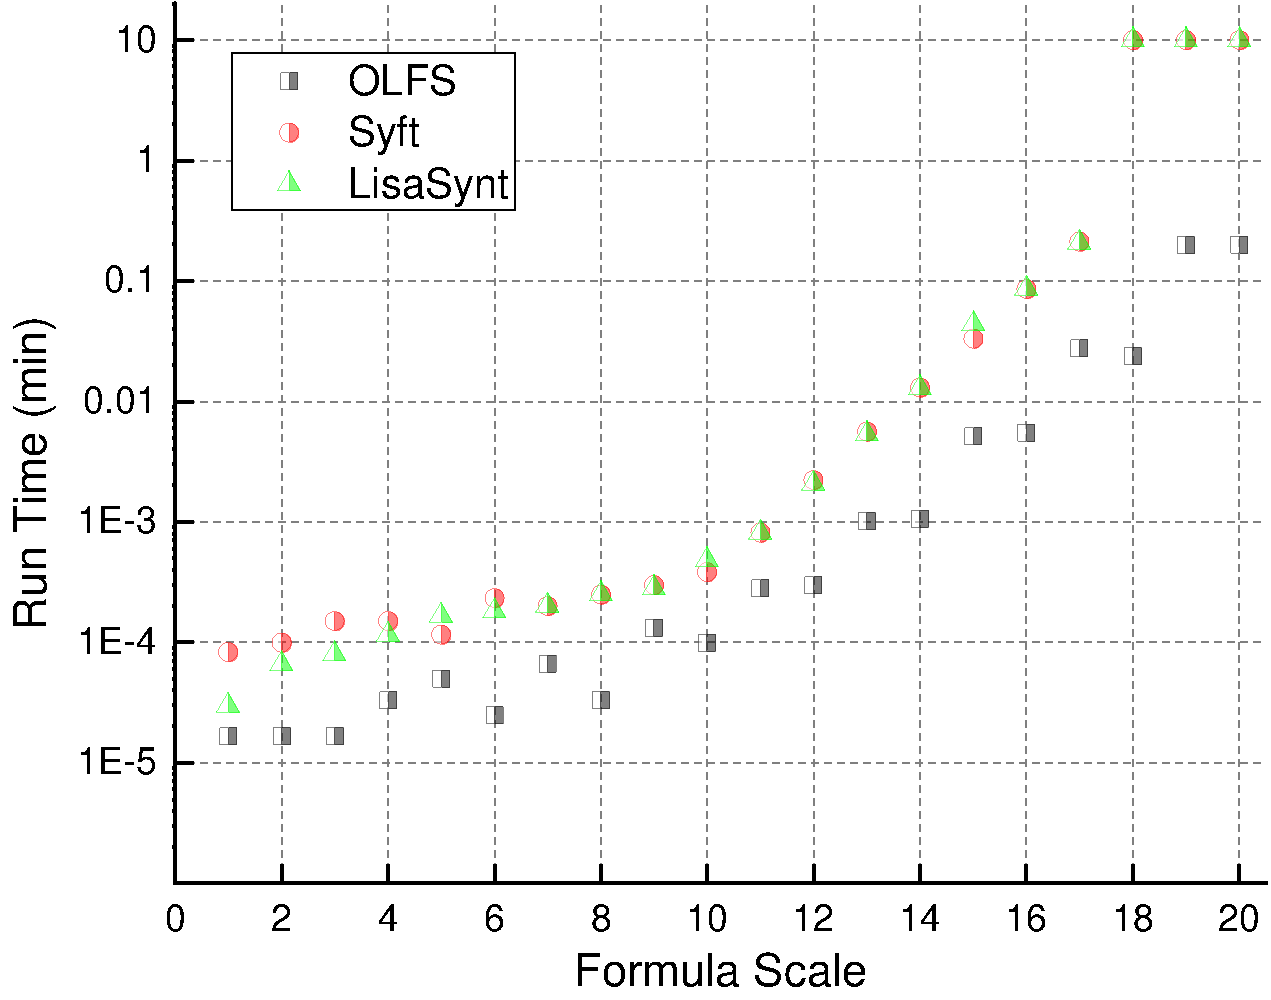
\includegraphics[width=5.5cm]{pic1_1.pdf}
    \caption{Results on the pattern formula $U (n) = p_1\U(p_2\U(...\U p_n))$.}
    \label{fig:preprocess-1}
\end{minipage}%
% }%
% \subfigure{
\begin{minipage}{0.33\linewidth}
\centering
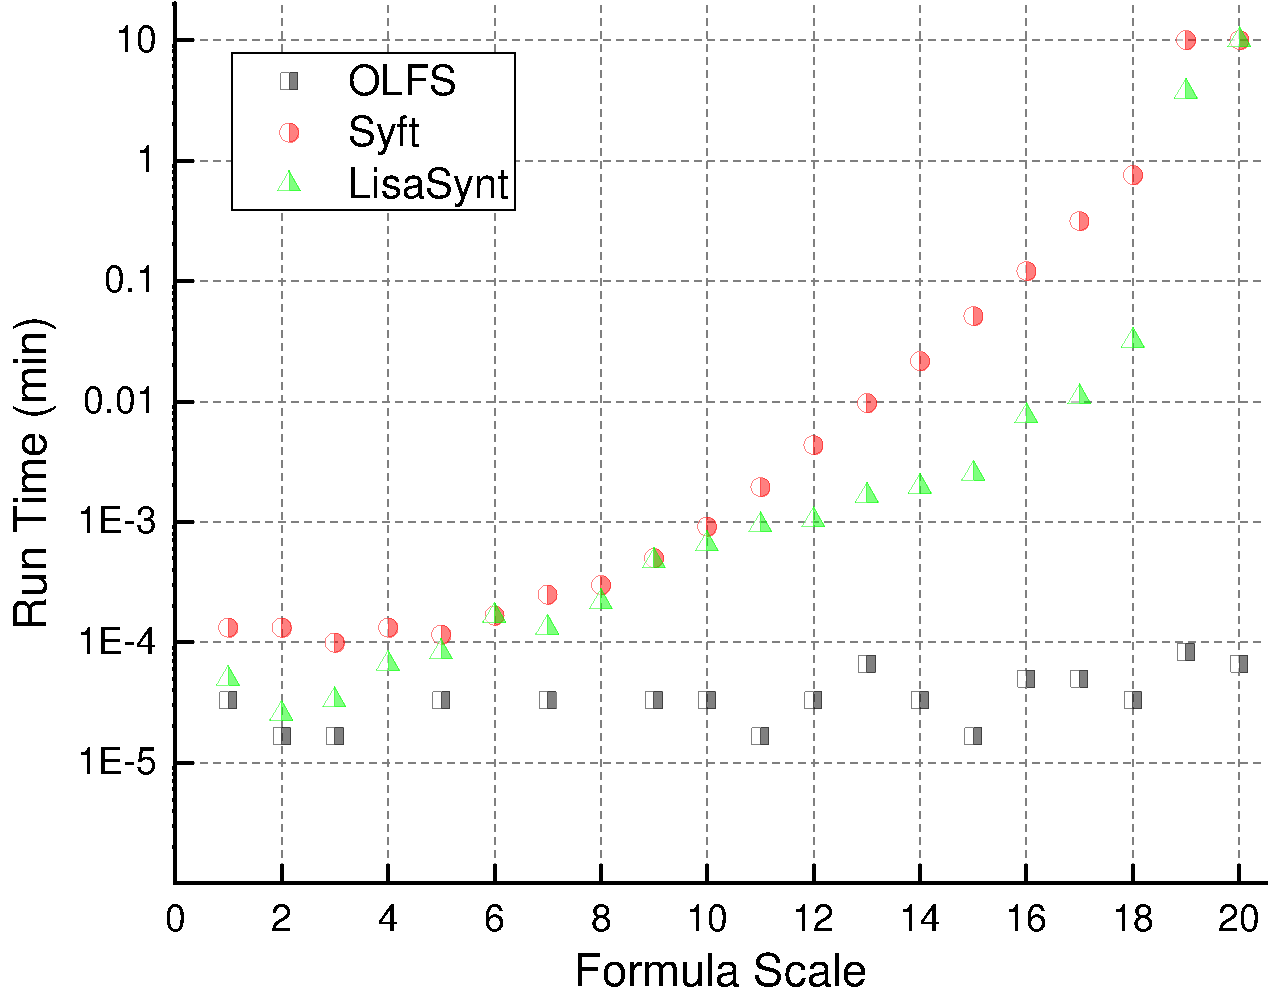
\includegraphics[width=5.5cm]{pic1_2.pdf}
    \caption{Results on the pattern formula $GF (n) = \G p_1\wedge(\bigwedge_{i=2\cdots n}\F p_i)$.}
    \label{fig:preprocess-2}
\end{minipage}%
% }%
% \subfigure{
\begin{minipage}{0.33\linewidth}
\centering
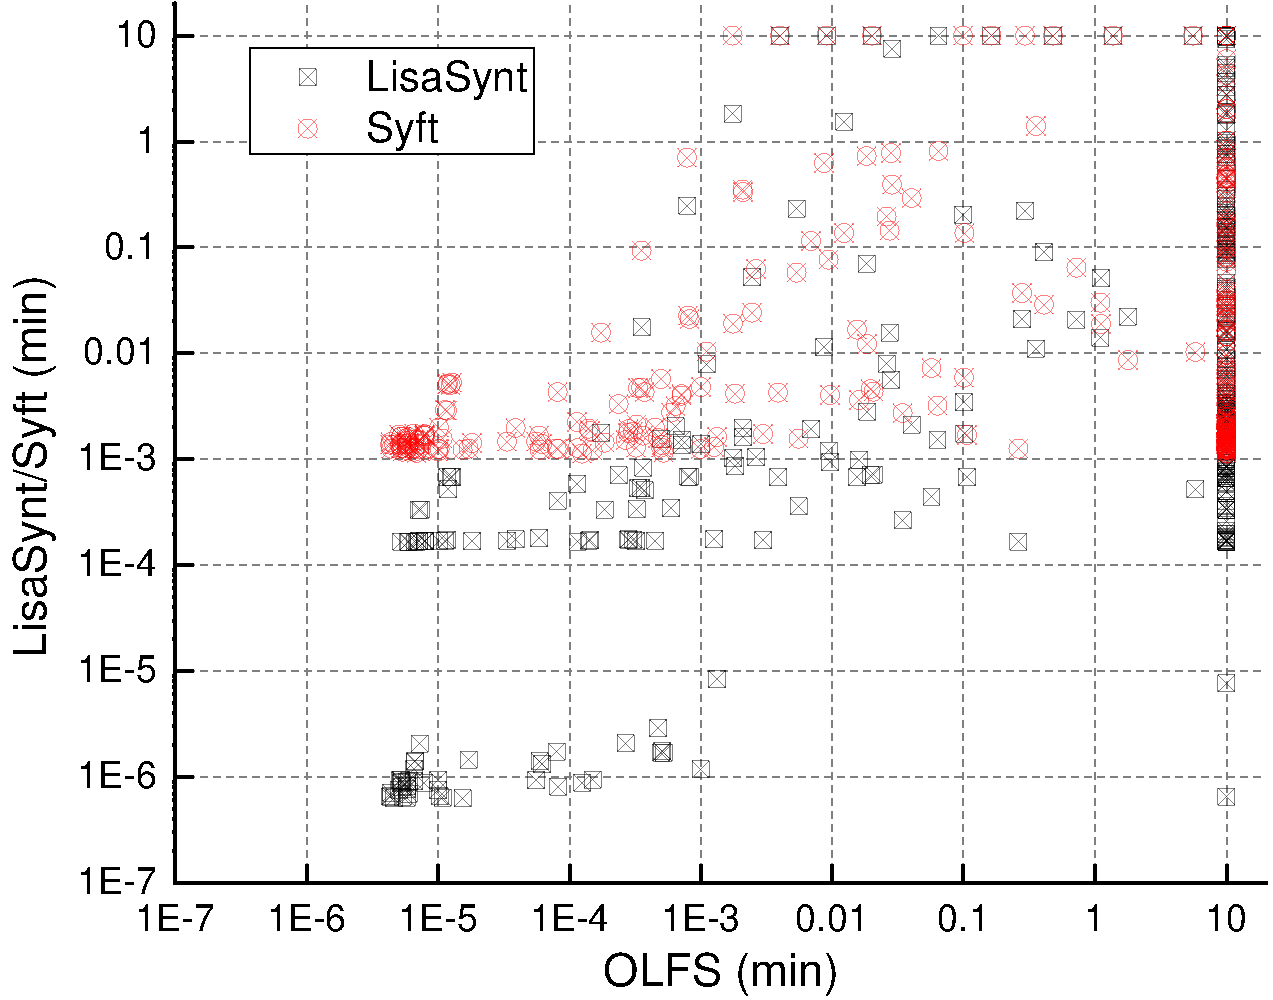
\includegraphics[width=5.5cm]{pic2.pdf}
    \caption{Results on the benchmarks from~\cite{BLTV20}.}
        \label{fig:otf}
\end{minipage}
% }%
\end{figure*}

Let $\Omega = \tool (\phi, \X, \Y)$ and we now define the strategy generator based on $\Omega$. Notably, our strategy generator only returns one winning strategy due to the on-the-fly construction, while the approach in \cite{GV15} is able to return all possible winning strategies. 

\begin{definition}[Strategy Generator]\label{def:transducer}
	The strategy generator for the \ltlf synthesis problem $(\phi, \X, \Y)$ is a transducer $\mathcal{T}_{\A}=(2^{\X\times\Y}, S, s_0, \xi, \sigma)$ such that
	\begin{itemize}
		\item $2^{\X\times\Y}$ is the alphabet of the transducer;
		\item $S = \{s| \langle s, Y, \{\langle X, s'\rangle\}\rangle \in\Omega\}\subseteq 2^{2^{\cl(\phi)}}$ is the set of states;
		\item $s_0 = \{\{\phi\}\}$ is the initial state;
		\item $\xi: S\times 2^{\X}\rightarrow 2^S$ is the transition function such that $\xi (s, X) = \{s' | \langle s, Y, \{\langle X, s'\rangle\}\rangle\in \Omega\}$;
		\item $\sigma: S\rightarrow 2^{\Y}$ is the output function such that $\sigma(s)=\{Y | \langle s, Y, \{\langle X, s'\rangle\}\rangle \in \Omega\}$.
	\end{itemize}
\end{definition}







%
\section {Experimental Evaluation}\label {sec:exp}

\noindent\textbf{Tools} We implemented both the pre-processing and on-the-fly synthesis techniques in the tool \toolname. We compared the results with extant \ltlf-synthesis tools \syft \cite{ZTLPV17} and \lisasyft \cite{BLTV20}. Both tools implement the synthesis approach proposed in \cite{GV15}, but distinguish with each other by using different complete \dfa constructions, monolithic and decompositional, respectively. All three tools were run with their default parameters. 

\noindent\textbf{Benchmarks}  We benchmark the experiment with the 430 instances presented in \cite{BLTV20}. We also select two classes of patterns $U$ and $GF$, which originate from~\cite{RV07} and are shown in Figure \ref{fig:preprocess-1} and Figure \ref{fig:preprocess-2} respectively, to test the efficiency of pre-processing techniques.

\noindent\textbf{Platform} We ran the experiments on a RedHat 6.0 cluster with 2304 processor cores
in 192 nodes (12 processor cores per node), running at 2.83 GHz with 48GB of
RAM per node. 
Each tool executed on a dedicated node with a timeout of 10 minutes, measuring execution time with Unix \texttt{time}. Excluding timeouts, all solvers found correct verdicts for all formulas. All artifacts are available in the supplemental materials.




\noindent\textbf{Results} Figure \ref{fig:preprocess-1} and Figure \ref{fig:preprocess-2} show the results on the $U$ and $GF$ patterns to evaluate the power of the pre-processing techniques presented in the paper. We carefully divide the atomic sets such that the synthesis on the $U$ pattern formulas are all realizable while the results for the $GF$ pattern formulas are all unrealizable. By applying Theorem \ref{thm:winning-1} to synthesis the $U$ patterns, \toolname is able to achieve a linear-cost performance. Meanwhile, \syft and \lisasyft reach the timeout when the pattern length $n$ is greater than 18 (see Figure \ref{fig:preprocess-1}). Analogously, Theorem \ref{thm:failure-1} enables \toolname to gain a linear-cost performance on the synthesis of the $GF$ patterns, while \syft and \lisasyft perform exponentially worse on such patterns (see Figure \ref{fig:preprocess-2}). 

Figure \ref{fig:otf} shows the comparison results between on-the-fly synthesis approach and the classical one presented in \cite{GV15}, represented by tools \syft and \lisasyft, on the 430 instances from \cite{BLTV20}. From the figure, the on-the-fly approach cannot outperform the classical one. In total, \toolname solves 149 out of 430 instances, while \syft and \lisasyft solve the number of 281 and 288 respectively. There are 50 of 149 instances for that \toolname can solve faster than the other two tools, as shown in Figure \ref{fig:otf}. Therefore, we conclude that the on-the-fly approach can complement the extant one. 

The reason why the current on-the-fly synthesis cannot perform better, is that a lot of time is consumed by the single \tdfa state generation. From Definition \ref{def:ltlf2dfa}, each state of the \tdfa belongs to $2^{2^{cl(\phi)}}$, where $\phi$ is the input formula. The \SAT-based technique shown in \cite{LRPZV19} is good at computing transitions for the \NFA, but the composition of the non-deterministic states so as to obtain the deterministic one is still over-loaded. From our experiments, we observe that most instances that cannot be solved by \toolname fall into this part. We leave the improvement of the on-the-fly synthesis to our future work.






\section {Experimental Evaluation}\label {sec:exp}

\noindent\textbf{Tools} We implemented both the pre-processing and on-the-fly synthesis techniques in the tool \toolname. We compared the results with extant \ltlf-synthesis tools \syft \cite{ZTLPV17} and \lisasyft \cite{BLTV20}. Both tools implement the synthesis approach proposed in \cite{GV15}, but distinguish with each other by using different complete \dfa constructions, monolithic and decompositional, respectively. All three tools were run with their default parameters. 

\noindent\textbf{Benchmarks}  We benchmark the experiment with the 430 instances presented in \cite{BLTV20}. We also select two classes of patterns $U$ and $GF$, which originate from~\cite{RV07} and are shown in Figure \ref{fig:preprocess-1} and Figure \ref{fig:preprocess-2} respectively, to test the efficiency of pre-processing techniques.

\noindent\textbf{Platform} We ran the experiments on a RedHat 6.0 cluster with 2304 processor cores
in 192 nodes (12 processor cores per node), running at 2.83 GHz with 48GB of
RAM per node. 
Each tool executed on a dedicated node with a timeout of 10 minutes, measuring execution time with Unix \texttt{time}. Excluding timeouts, all solvers found correct verdicts for all formulas. All artifacts are available in the supplemental materials.




\noindent\textbf{Results} Figure \ref{fig:preprocess-1} and Figure \ref{fig:preprocess-2} show the results on the $U$ and $GF$ patterns to evaluate the power of the pre-processing techniques presented in the paper. We carefully divide the atomic sets such that the synthesis on the $U$ pattern formulas are all realizable while the results for the $GF$ pattern formulas are all unrealizable. By applying Theorem \ref{thm:winning-1} to synthesis the $U$ patterns, \toolname is able to achieve a linear-cost performance. Meanwhile, \syft and \lisasyft reach the timeout when the pattern length $n$ is greater than 18 (see Figure \ref{fig:preprocess-1}). Analogously, Theorem \ref{thm:failure-1} enables \toolname to gain a linear-cost performance on the synthesis of the $GF$ patterns, while \syft and \lisasyft perform exponentially worse on such patterns (see Figure \ref{fig:preprocess-2}). 

Figure \ref{fig:otf} shows the comparison results between on-the-fly synthesis approach and the classical one presented in \cite{GV15}, represented by tools \syft and \lisasyft, on the 430 instances from \cite{BLTV20}. From the figure, the on-the-fly approach cannot outperform the classical one. In total, \toolname solves 149 out of 430 instances, while \syft and \lisasyft solve the number of 281 and 288 respectively. There are 50 of 149 instances for that \toolname can solve faster than the other two tools, as shown in Figure \ref{fig:otf}. Therefore, we conclude that the on-the-fly approach can complement the extant one. 

The reason why the current on-the-fly synthesis cannot perform better, is that a lot of time is consumed by the single \tdfa state generation. From Definition \ref{def:ltlf2dfa}, each state of the \tdfa belongs to $2^{2^{cl(\phi)}}$, where $\phi$ is the input formula. The \SAT-based technique shown in \cite{LRPZV19} is good at computing transitions for the \NFA, but the composition of the non-deterministic states so as to obtain the deterministic one is still over-loaded. From our experiments, we observe that most instances that cannot be solved by \toolname fall into this part. We leave the improvement of the on-the-fly synthesis to our future work.






%\section{Discussion and Concluding Remarks}\label{sec:con}


\section{Concluding Remarks}\label{sec:con}

In this paper, we present both the pre-processing and on-the-fly techniques to solve the synthesis problem of \ltl over finite traces. Comparing to existing methods, our approach allows us to perform the synthesis by possibly just generating partially the \dfa w.r.t. the input \ltlf formula. The experiment results show that, (1) the pre-processing technique can bring an exponential-better performance than the classical synthesis approach; (2) our on-the-fly synthesis approach complements the extant one by speeding up the synthesis of 50 instances in the benchmarks.  




%\newpage
\section{Acknowledgment}
%We thank anonymous reviewers for useful comments. 
Jianwen Li and Geguang Pu are supported by  Science and Technology Commitment of Shanghai (\#20PJ1403500 and \#19511103602), NSFC (\#62002118, \#61632005 and \#61532019) and National Key Research and Development Program (\#2020AAA0107800). Shufang Zhu is supported by ERC Advanced Grant (\#834228) and EU ICT-48 2020 project (\#952215). Moshe Vardi is supported by NSF grants IIS-1527668, CCF-1704883,
IIS-1830549, and an award from the Maryland Procurement Office.

%\bibliographystyle{aaai21}
\bibliography{ok,cav}

%\newpage
%\section{Appendix}
\subsection{Proof of Theorem \ref{thm:ltlf2tdfa}}

We first introduce the following lemma to prove Theorem \ref{thm:ltlf2tdfa}.

\begin{lemma}\label{lem:propSat}
Given an \ltlf formula $\phi$ in the \XNF and a finite trace $\eta\in\Sigma^+$ with $|\eta|>1$, $\eta\models\phi$ holds iff there is a satisfying assignment $A$ of $\phi$ such that $\eta[0]\models L(A)$ and $\eta_1\models X(A)$.
\end{lemma}
\begin{proof}
$(\Rightarrow)$ The proof can be achieved by induction over the types of $\phi$. Since $\phi$ is in \XNF, $\phi$ cannot be an Until or Release formula.
\begin{itemize}
	\item if $\phi$ is a literal,  we could have a satisfying assignment $A=\{\phi\}$ for $\phi$. In this situation, $L(A)=\{\phi\}$ and $X(A)=\{\tt\}$. Therefore, it is true that $\eta[0]\models L(A)$ and $\eta_1\models X(A)$;
	\item if $\phi=\X\psi$, we could have a satisfying assignment $A=\{\X\psi\}$ for $\phi$. In this situation, $L(A)=\{\tt\}$ and $X(A)=\{\psi\}$. Considering we have $\eta\models\phi$ i.e., $\eta\models\X\psi$, it is true that $\eta[0]\models L(A)$ and $\eta_1\models X(A)$;
	\item if $\phi = \phi_1\wedge\phi_2$, $\eta\models\phi$ 
implies $\eta\models\phi_1$ and $\eta\models\phi_2$. By assumption hypothesis, there is $A_i$ of $\phi_i$ ($i=1,2$) such that 
$\eta[0]\models L(A_i)$ and $\eta_1\models X(A_i)$. Let $A = A_1\cup A_2$, and a consistent $A$, in which either $\psi$ or $\neg \psi$ cannot be together, 
must exists ($A$ may not be unique because $A_1$ and $A_2$ may not be unique). 
Otherwise, there is $\psi\in A_1$ and $\neg\psi\in A_2$ 
such that $\eta$ cannot model $\bigwedge A_1$ and $\bigwedge A_2$ at the same time, which is a contradiction. So $A$ is a satisfying  assignment of $\phi$, which leads to $\eta[0]\models L(A)$ and $\eta_1\models X(A)$. 
\item The proof for $\phi=\phi_1\vee\phi_2$ is analogous to the proof for $\phi = \phi_1\wedge\phi_2$.
\end{itemize} 

$(\Leftarrow)$ Let $A$ be a satisfying assignment of $\phi$, so $A\models\phi$ implies $(\bigwedge A)\Rightarrow \phi$. 
Also, $\eta[0]\models L(A)$ and $\eta_1\models X(A)$ implies $\eta\models \bigwedge A$. Therefore, it is true that $\eta\models \phi$.
\end{proof}

Lemma \ref{lem:propSat} does not cover the case when $|\eta|=1$, which yields the following corollary. 

\begin{corollary}\label{coro:propSat}
Given an \ltlf formula $\phi$ in the \XNF and a finite trace $\eta\in\Sigma^+$ with $|\eta|=1$, $\eta\models\phi$ holds implies there is a satisfying assignment $A$ of $\phi$ such that $\eta[0]\models L(A)$.
\end{corollary}
\begin{proof}
The proof is similar to that of Lemma \ref{lem:propSat} for the ($\Rightarrow$) direction, the details of which are omitted here.
\end{proof}

Now we start to prove Theorem \ref{thm:ltlf2tdfa}
\iffalse
\begin{theorem}
Given an \ltlf formula $\phi$ and the \TDFA ${\A_{\phi}}$ constructed by Definition \ref{def:ltlf2dfa}, a finite trace $\eta\models\phi$ holds iff $\eta$ is accepted by ${\A_{\phi}}$. 
\end{theorem}
\fi
\begin{proof}
Assume $\eta = \omega_0\omega_1\ldots\omega_n$ ($n\geq 0$). 

($\Leftarrow$) 
According to Definition \ref{def:ltlf2dfa},  $\eta$ accepted by ${\A_{\phi}}$ implies that there is a run $r=s_0s_1\ldots s_n s_{n+1}$ of ${\A_{\phi}}$ on $\eta$ such that $s_{n}\tran{\omega_{n}}s_{n+1} \in \delta$ and $\omega_n\models s_n$. To prove $\eta$ is accepted by ${\A_{\phi}}$ implies $\eta\models\phi$ holds, we only need to prove $\eta$ is accepted by ${\A_{\phi}}$ implies $\eta_{n-i}\models s_{n-i}$ for\ i=0...n. Then we could have $\eta (=\eta_0)\models \phi (=s_0)$ when $i=n$.

We prove by induction over the values of $i$.
\begin{itemize}
	\item By Definition \ref{def:ltlf2dfa}, we have that $\omega_n\models s_n$, which means basically when $i = 0$, it holds that $\eta_{n-0}\models s_{n-0}$;
	\item Inductively, assume $\eta_{n-i}\models s_{n-i}$ holds($0<i\leq n$). Because $s_{n-i-1}\tran{\omega_{n-i-1}}s_{n-i}$ is a transition in the \TDFA and $\eta_{n-i}\models s_{n-i}$ holds, the set $A_{n-i-1} = \omega_{n-i-1}\cup \{\X\theta | \theta\in s\}$ is a satisfying assignment of $\xnf{s_{n-i-1}}$ in $\SAT(\xnf{s_{n-i-1}})$, from Definition \ref{def:ltlf2dfa}. Then based on Lemma \ref{lem:propSat} and since $\eta_{n-i-1}=\omega_{n-i-1}\cdot\eta_{n-i}$ is true, we have that $\eta_{n-i-1}\models s_{n-i-1}$.
\end{itemize}

($\Rightarrow$) We first prove that $\eta\models\phi$ implies that there is a run $r$ of ${\A_{\phi}}$ on $\eta$. 
If $n = 0$, Corollary \ref{coro:propSat} shows that there is a satisfying assignment $A$ of $\xnf{\phi}$ such that $\eta[0]\models L(A)$. From Definition \ref{def:ltlf2dfa}, $\phi\tran{\eta[0]}s$, where $s=\{X(A') | A'\in\SAT(\xnf{\phi})\}$, is a transition of the \TDFA. As a result, there is a run $r=s_0(=\phi)s$ of ${\A_{\phi}}$ on $\eta$.
 
If $n>0$, according to Lemma \ref{lem:propSat}, $\eta\models\phi$ implies there is a satisfying assignment $A$ of $\xnf{\phi}$ such that $\omega_0\models L(A)$ and $\eta_1\models X(A)$. From Definition \ref{def:ltlf2dfa}, $\phi (=s_0)\tran{\omega_0}s_1$, where $s_1=\{X(A') | A'\in\SAT(\xnf{\phi})\}$, is a transition in the \TDFA. Recursively applying the above process to $\eta_i\models s_i(i\geq 1)$, one can prove there is a transition $s_i\tran{\omega_i}s_{i+1}$ in the \TDFA. As a result, we have $\eta\models\phi$, which implies there is a run $r$ of ${\A_{\phi}}$ on $\eta$.  

Now we have that $\eta\models\phi$ implies there is a run $r=s_0...s_n s_{n+1}$ of ${\A_{\phi}}$ on $\eta$ and $\eta_i\models s_i\ for\ i=0...n$. When $i=n$, $\eta_n\models s_n$ i.e., $\omega_n\models s_n$ holds. According to Definition \ref{def:ltlf2dfa}, the transition $s_n\tran{\omega_n}s_{n+1}$ is an accepting transition. As a result, $r$ is an accepting run and $\eta$ is accepted by ${\A_{\phi}}$.
\end{proof}




\end{document}
